\documentclass[10pt]{article}
\usepackage[preprint]{tmlr}
% Camera-ready: \usepackage[accepted]{tmlr}   Preprint: \usepackage[preprint]{tmlr}
\usepackage[utf8]{inputenc}
\usepackage[T1]{fontenc}
\usepackage{amsmath,amssymb,amsthm,bm}
\usepackage{graphicx}
\usepackage{booktabs,multirow}
\usepackage{algorithm}
\usepackage{algpseudocode}
\usepackage{tikz}
\usetikzlibrary{arrows.meta,positioning,fit,calc,shapes.geometric}
\usepackage{xcolor}
\usepackage{url}
\usepackage{hyperref}

\newtheorem{proposition}{Proposition}
\newtheorem{lemma}{Lemma}
\newtheorem{assumption}{Assumption}
\newtheorem{remark}{Remark}
\newtheorem{corollary}{Corollary}
\DeclareMathOperator*{\argmax}{arg\,max}
\newcommand{\zh}{\hat{z}}
\newcommand{\zt}{\tilde{z}}
\newcommand{\Up}{\mathrm{Up}}
\newcommand{\KL}{D_{\mathrm{KL}}}
\newcommand{\OffEasy}{99.40}
\newcommand{\BaseEasy}{99.47}
\newcommand{\LoopVoneEasy}{58.17}
\newcommand{\OffMedium}{96.40}
\newcommand{\BaseMedium}{96.00}
\newcommand{\LoopVoneMedium}{78.03}
\newcommand{\OffHard}{86.30}
\newcommand{\BaseHard}{86.67}
\newcommand{\LoopVoneHard}{24.19}
\newcommand{\OffWmt}{21.72}
\newcommand{\OffXsumRone}{34.68}
\newcommand{\OffXsumRtwo}{12.55}
\newcommand{\OffXsumRL}{27.69}
\newcommand{\BaseXsum}{27.62}
\newcommand{\LoopVoneXsum}{6.25}
\newcommand{\BaseWmt}{22.35}
\newcommand{\LoopVoneWmt}{0.21}
\newcommand{\LDSud}{0.026}
\newcommand{\LDWmt}{0.073}
\newcommand{\RhoGtOneSud}{8}
\newcommand{\RhoGtOneWmt}{6}
\newcommand{\FluxLastSud}{0.50}
\newcommand{\FluxLastWmt}{0.30}
\newcommand{\CorrParams}{1.23}
\newcommand{\ZsFluxFiveHard}{27.4}
\newcommand{\ZsFluxFiveLevHard}{7.24}
\newcommand{\ZsStabTenHard}{77.5}
\newcommand{\ZsStabTenLevHard}{11.27}
\newcommand{\ZsBaseHard}{86.3}
\newcommand{\ZsFluxFiveMedium}{96.4}
\newcommand{\ZsFluxFiveLevMedium}{12.00}
\newcommand{\ZsStabTenMedium}{96.4}
\newcommand{\ZsStabTenLevMedium}{12.00}
\newcommand{\ZsBaseMedium}{96.4}
\newcommand{\ZsFluxFifteenMedium}{18.7}
\newcommand{\ZsFluxFifteenLevMedium}{4.86}
\newcommand{\LoopVtwoHard}{86.79}
\newcommand{\LoopVtwoHardStd}{0.17}
\newcommand{\LoopVtwoHardP}{0.454}
\newcommand{\LoopVtwoHardT}{0.181}
\newcommand{\ProjNCM}{84.4}
\newcommand{\ProjNoSelOff}{6.2}
\newcommand{\ProjNoSelOn}{81.2}
\newcommand{\ProjSelOff}{84.4}
\newcommand{\ProjSelOn}{84.4}
\newcommand{\MarginEqMax}{0}
\newcommand{\MarginMedMax}{0.016}
\newcommand{\FlipsMin}{10.7}
\newcommand{\FlipsMax}{15.7}
\newcommand{\DgTfEasy}{98.96}
\newcommand{\DgPTfEasy}{0.002}
\newcommand{\DgDagEasy}{98.92}
\newcommand{\DgPDagEasy}{5.1e-04}
\newcommand{\DgDagCEasy}{99.04}
\newcommand{\DgPDagCEasy}{0.002}
\newcommand{\DgTfMedium}{95.93}
\newcommand{\DgPTfMedium}{0.266}
\newcommand{\DgDagMedium}{95.75}
\newcommand{\DgPDagMedium}{0.261}
\newcommand{\DgDagCMedium}{95.75}
\newcommand{\DgPDagCMedium}{0.162}
\newcommand{\DgTfHard}{85.87}
\newcommand{\DgPTfHard}{0.178}
\newcommand{\DgDagHard}{86.27}
\newcommand{\DgPDagHard}{0.197}
\newcommand{\DgDagCHard}{86.27}
\newcommand{\DgPDagCHard}{0.404}
\newcommand{\WmtMseLo}{0.90}
\newcommand{\WmtMseHi}{1.00}
\newcommand{\WmtUncLo}{1.19}
\newcommand{\WmtUncHi}{1.37}

\newcommand{\CzeroSud}{-0.15}
\newcommand{\CzeroWmt}{0.08}
\newcommand{\LGSud}{0.18}
\newcommand{\LGWmt}{0.12}
\newcommand{\SigOnSud}{6.1}
\newcommand{\SigOneSud}{8.9}
\newcommand{\DistZeroSud}{0.6}
\newcommand{\DistOneSud}{11.0}
\newcommand{\SigOnWmt}{36.1}
\newcommand{\SigOneWmt}{36.3}

\newcommand{\VfBaseEasy}{99.47}
\newcommand{\VfLoopEasy}{97.12}
\newcommand{\VfLoopEasyStd}{3.68}
\newcommand{\VfLoopEasyP}{0.23}
\newcommand{\VfLoopEasyMin}{90.87}
\newcommand{\VfLoopEasyMax}{99.53}
\newcommand{\VfLoopSelEasy}{99.49}
\newcommand{\VfLoopSelEasyStd}{0.08}
\newcommand{\VfLoopSelEasyP}{0.48}
\newcommand{\VfLoopSelEasyMin}{99.40}
\newcommand{\VfLoopSelEasyMax}{99.60}
\newcommand{\VfProjEasy}{99.61}
\newcommand{\VfProjEasyStd}{0.10}
\newcommand{\VfProjEasyP}{0.03}
\newcommand{\VfProjEasyMin}{99.47}
\newcommand{\VfProjEasyMax}{99.73}
\newcommand{\VfProjSelEasy}{99.53}
\newcommand{\VfProjSelEasyStd}{0.12}
\newcommand{\VfProjSelEasyP}{0.27}
\newcommand{\VfProjSelEasyMin}{99.47}
\newcommand{\VfProjSelEasyMax}{99.73}
\newcommand{\VfSzeroEasy}{1}
\newcommand{\VfBaseMed}{96.00}
\newcommand{\VfLoopMed}{90.77}
\newcommand{\VfLoopMedStd}{6.07}
\newcommand{\VfLoopMedP}{0.13}
\newcommand{\VfLoopMedMin}{79.93}
\newcommand{\VfLoopMedMax}{94.00}
\newcommand{\VfLoopSelMed}{96.27}
\newcommand{\VfLoopSelMedStd}{0.36}
\newcommand{\VfLoopSelMedP}{0.17}
\newcommand{\VfLoopSelMedMin}{95.80}
\newcommand{\VfLoopSelMedMax}{96.67}
\newcommand{\VfProjMed}{95.75}
\newcommand{\VfProjMedStd}{0.24}
\newcommand{\VfProjMedP}{0.08}
\newcommand{\VfProjMedMin}{95.33}
\newcommand{\VfProjMedMax}{95.93}
\newcommand{\VfProjSelMed}{95.92}
\newcommand{\VfProjSelMedStd}{0.03}
\newcommand{\VfProjSelMedP}{0.004}
\newcommand{\VfProjSelMedMin}{95.87}
\newcommand{\VfProjSelMedMax}{95.93}
\newcommand{\VfSzeroMed}{1}
\newcommand{\VfBaseHard}{86.67}
\newcommand{\VfLoopHard}{83.92}
\newcommand{\VfLoopHardStd}{4.07}
\newcommand{\VfLoopHardP}{0.21}
\newcommand{\VfLoopHardMin}{77.27}
\newcommand{\VfLoopHardMax}{86.80}
\newcommand{\VfLoopSelHard}{87.00}
\newcommand{\VfLoopSelHardStd}{0.16}
\newcommand{\VfLoopSelHardP}{0.01}
\newcommand{\VfLoopSelHardMin}{86.80}
\newcommand{\VfLoopSelHardMax}{87.20}
\newcommand{\VfProjHard}{86.63}
\newcommand{\VfProjHardStd}{0.23}
\newcommand{\VfProjHardP}{0.72}
\newcommand{\VfProjHardMin}{86.40}
\newcommand{\VfProjHardMax}{87.00}
\newcommand{\VfProjSelHard}{86.47}
\newcommand{\VfProjSelHardStd}{0.00}
\newcommand{\VfProjSelHardP}{1.00}
\newcommand{\VfProjSelHardMin}{86.47}
\newcommand{\VfProjSelHardMax}{86.47}
\newcommand{\VfSzeroHard}{0}
\newcommand{\VfBaseWmt}{21.72}
\newcommand{\VfLoopWmt}{1.45}
\newcommand{\VfLoopWmtStd}{1.76}
\newcommand{\VfLoopWmtP}{$<\!10^{-4}$}
\newcommand{\VfLoopWmtMin}{0.44}
\newcommand{\VfLoopWmtMax}{4.59}
\newcommand{\VfLoopSelWmt}{21.72}
\newcommand{\VfLoopSelWmtStd}{0.00}
\newcommand{\VfLoopSelWmtP}{1.00}
\newcommand{\VfLoopSelWmtMin}{21.72}
\newcommand{\VfLoopSelWmtMax}{21.72}
\newcommand{\VfProjWmt}{2.52}
\newcommand{\VfProjWmtStd}{0.53}
\newcommand{\VfProjWmtP}{$<\!10^{-4}$}
\newcommand{\VfProjWmtMin}{1.90}
\newcommand{\VfProjWmtMax}{3.22}
\newcommand{\VfProjSelWmt}{15.82}
\newcommand{\VfProjSelWmtStd}{0.00}
\newcommand{\VfProjSelWmtP}{1.00}
\newcommand{\VfProjSelWmtMin}{15.82}
\newcommand{\VfProjSelWmtMax}{15.82}
\newcommand{\VfSzeroWmt}{5}
\newcommand{\VfBaseXsum}{27.64}
\newcommand{\VfLoopXsum}{11.87}
\newcommand{\VfLoopXsumStd}{0.96}
\newcommand{\VfLoopXsumP}{$<\!10^{-4}$}
\newcommand{\VfLoopXsumMin}{10.54}
\newcommand{\VfLoopXsumMax}{13.08}
\newcommand{\VfLoopSelXsum}{27.64}
\newcommand{\VfLoopSelXsumStd}{0.00}
\newcommand{\VfLoopSelXsumP}{1.00}
\newcommand{\VfLoopSelXsumMin}{27.64}
\newcommand{\VfLoopSelXsumMax}{27.64}
\newcommand{\VfProjXsum}{20.07}
\newcommand{\VfProjXsumStd}{0.40}
\newcommand{\VfProjXsumP}{$<\!10^{-4}$}
\newcommand{\VfProjXsumMin}{19.44}
\newcommand{\VfProjXsumMax}{20.54}
\newcommand{\VfProjSelXsum}{27.56}
\newcommand{\VfProjSelXsumStd}{0.10}
\newcommand{\VfProjSelXsumP}{0.15}
\newcommand{\VfProjSelXsumMin}{27.39}
\newcommand{\VfProjSelXsumMax}{27.61}
\newcommand{\VfSzeroXsum}{5}
\newcommand{\VaDagHard}{87.16}
\newcommand{\VaDagHardStd}{0.53}
\newcommand{\VaDagHardP}{0.11}
\newcommand{\VaDagHardMax}{88.07}
\newcommand{\VaDagHardMinP}{0.02}
\newcommand{\VaDagHardKept}{0}
\newcommand{\VaDagCHard}{87.13}
\newcommand{\VaDagCHardStd}{0.53}
\newcommand{\VaDagCHardP}{0.12}
\newcommand{\VaDagCHardMax}{87.80}
\newcommand{\VaDagCHardMinP}{0.07}
\newcommand{\VaDagCHardKept}{0}
\newcommand{\VaDagMedium}{95.71}
\newcommand{\VaDagMediumStd}{0.27}
\newcommand{\VaDagMediumP}{0.07}
\newcommand{\VaDagMediumMax}{96.00}
\newcommand{\VaDagMediumMinP}{0.29}
\newcommand{\VaDagMediumKept}{2}
\newcommand{\VaDagCMedium}{95.92}
\newcommand{\VaDagCMediumStd}{0.17}
\newcommand{\VaDagCMediumP}{0.36}
\newcommand{\VaDagCMediumMax}{96.13}
\newcommand{\VaDagCMediumMinP}{0.59}
\newcommand{\VaDagCMediumKept}{1}
\newcommand{\PrHardLab}{0.0}
\newcommand{\PrHardLev}{12.00}
\newcommand{\PrHardQ}{86.67}
\newcommand{\PrHardFull}{86.67}
\newcommand{\PrHardSave}{0.00}
\newcommand{\PrMedLab}{0.0}
\newcommand{\PrMedLev}{12.00}
\newcommand{\PrMedQ}{96.00}
\newcommand{\PrMedFull}{96.00}
\newcommand{\PrMedSave}{0.00}
\newcommand{\PrEasyLab}{0.0}
\newcommand{\PrEasyLev}{12.00}
\newcommand{\PrEasyQ}{99.47}
\newcommand{\PrEasyFull}{99.47}
\newcommand{\PrEasySave}{0.00}
\newcommand{\PrXsumLab}{4.3}
\newcommand{\PrXsumLev}{8.96}
\newcommand{\PrXsumQ}{27.60}
\newcommand{\PrXsumFull}{27.64}
\newcommand{\PrXsumSave}{0.04}
\newcommand{\PrXsumAuc}{0.86}
\newcommand{\PtBaseVal}{82.4}
\newcommand{\PtFiveMax}{78.9}
\newcommand{\PtTenMax}{79.1}
\newcommand{\PtMin}{77.5}
\newcommand{\PtLoopSelMin}{86.67}
\newcommand{\PtLoopSelMax}{87.07}
\newcommand{\PtLoopOneMin}{75.1}
\newcommand{\PtLoopOneMax}{81.0}


\title{Why Post-Hoc Latent Revision and Adaptive Halting Fail on Frozen Coarse-to-Fine Language Models: Theoretical Conditions and Empirical Diagnostics}

% Authors are hidden automatically in the anonymous submission mode.
\author{\name S M Tasfik Us Salahin \email TashfikS@users.noreply.github.com}

\def\month{MM}
\def\year{YYYY}
\def\openreview{\url{https://openreview.net/forum?id=XXXX}}

\begin{document}
\maketitle

\begin{abstract}
Coarse-to-fine next-concept models (NCM) generate text by emitting one level of a multiscale residual vector quantizer (MS-RVQ) per parallel step. Two training-free extensions seem natural for such models: predictor-corrector revision of the cumulative latent, borrowed from score-based diffusion samplers, and adaptive early halting, motivated by the nested fine-drop training that makes intermediate latents decodable. We ask whether either can improve a frozen NCM. We first derive the conditions under which each mechanism can succeed: a corrector reduces accumulated drift only if it is contractive \emph{in closed loop} on the generator's support (Proposition~1), and halting at level $k^\ast$ bounds the output KL divergence by $L_D^2\tau^2/(2(1-\rho)^2)$ only if latent increments decay geometrically with $\rho<1$ and the final decoding has margin (Proposition~2). We then test these conditions on five official NCM checkpoints (Sudoku easy/medium/hard, WMT14 De--En, XSum) with a bit-exact harness, five seeds and paired tests, and identify three properties of standard MS-RVQ pre-training that violate them. (i) Off-manifold exposure bias: continuous correction lowers open-loop latent error on WMT14 (\WmtMseLo--\WmtMseHi{} vs.\ \WmtUncLo--\WmtUncHi) yet collapses generation (Sudoku-hard \LoopVoneHard\%, WMT14 \LoopVoneWmt{} BLEU, XSum \LoopVoneXsum{} ROUGE-L); codebook projection removes most of the collapse but does not beat NCM, and DAgger fine-tuning of the generator gives no significant gain (and a significant loss on Sudoku-easy, where validation is saturated). (ii) Non-decaying flux: $\hat\rho>1$ on \RhoGtOneSud{}/10 Sudoku-hard and \RhoGtOneWmt{}/9 WMT14 transitions. (iii) Terminal-level concentration: no Sudoku board's intermediate decoding equals its final one, so even per-sequence margin halting cannot exit early. We conclude with pre-training prescriptions that would satisfy both propositions.
\end{abstract}


\section{Introduction}
Autoregressive (AR) Transformers~\citep{vaswani2017attention,radford2019language,brown2020language} generate one token per network evaluation, so latency grows linearly with output length. Two families of parallel generators have been proposed to remove this bottleneck. Non-autoregressive and iterative-refinement models~\citep{gu2018nat,lee2018deterministic,ghazvininejad2019maskpredict,gu2019levenshtein} and, more recently, discrete diffusion language models (DLMs)~\citep{austin2021d3pm,li2022diffusionlm,lou2024sedd,sahoo2024mdlm,shi2024md4,gulrajani2023plaid,nie2025llada} predict many tokens per step, but they revisit the full sequence at every step and degrade quickly when the number of steps is reduced. Next-Concept Modeling (NCM)~\citep{kumbong2026ncm} takes a third route that is closer to next-scale prediction in vision~\citep{tian2024var}: a multiscale residual VQ-VAE (MS-RVQ) encodes a sequence into $K$ levels of discrete codes of increasing length, and a Transformer generates one level per forward pass, emitting all codes within a level in parallel. On the released checkpoints, NCM solves 99.4\% of easy Sudoku boards with 12 network evaluations and is 10--31$\times$ faster than diffusion baselines on text~\citep{kumbong2026ncm}.

Two structural properties of NCM motivate this work. First, the latent state is \emph{purely additive}: the cumulative reconstruction after level $k$ is the sum of the upsampled code embeddings of levels $0,\dots,k$, and nothing in the sampler can revise a coarse code once it has been emitted. A wrong code at a coarse level, where a single position covers many output tokens, is broadcast over the whole sequence by linear interpolation, and finer codebooks, which were fitted to \emph{clean} residuals, are evaluated out of distribution. Second, the depth of generation is \emph{fixed}: every input pays for all $K$ levels, although the official tokenizers are trained with fine-level dropout (\texttt{fine\_drop}), a nested-dropout scheme~\citep{rippel2014nested} that makes intermediate cumulative latents decodable by the frozen decoder.

These observations suggest two training-free modifications borrowed from continuous-time samplers and adaptive-computation networks: a learned \emph{corrector} that revises the cumulative latent after every predictor step, as in predictor-corrector diffusion samplers~\citep{song2021sde,zhao2023unipc}, and a \emph{halting rule} that stops generation once the latent has converged, as in adaptive computation time and early-exit Transformers~\citep{graves2016act,banino2021pondernet,elbayad2020depth,schuster2022calm}. We call the combination Adaptive Predictor-Corrector NCM (APC-NCM). The central question of this paper is: \emph{can predictor-corrector latent revision and adaptive early halting improve a frozen coarse-to-fine NCM without retraining it?} We answer it in two parts. We first derive the conditions each mechanism requires, then test these conditions on the released checkpoints under a strict protocol: official code, no access to targets at inference, hyper-parameters selected only on held-out inputs, five seeds, and paired significance tests. The answer is negative, and the analysis identifies why.

Our contributions are:
\begin{itemize}
\item \textbf{Formulation.} We write the NCM sampler as a predictor that adds one quantized residual per level, formalize the additive-drift failure mode, and define a learned latent corrector $C_\omega$ applied in the loop, on the decode path, or with projection back onto the codebook lattice, as well as batch-level and per-sequence halting rules.
\item \textbf{Conditions for success.} Proposition~\ref{prop:contraction} shows that additive MS-RVQ error grows linearly in the per-level code error, whereas a corrector that is $\epsilon_{\mathrm{corr}}$-accurate and contractive along the \emph{closed-loop} trajectory yields a bounded error governed by $\prod_j(1-\gamma_j)$. Proposition~\ref{prop:rd} bounds the KL cost of halting by $L_D^2\tau^2/(2(1-\rho)^2)$ under geometric increment decay $\rho<1$, and a Pinsker argument turns this into exact output preservation when the final decoding has sufficient margin.
\item \textbf{Bit-exact controlled evaluation.} We reproduce the official baselines on a T4 (Sudoku easy/medium/hard: \OffEasy/\OffMedium/\OffHard\% solved; WMT14 De--En: \OffWmt{} BLEU; XSum: \OffXsumRL{} ROUGE-L) with a harness that wraps the official sampler unchanged, and evaluate every variant with 5 seeds, Wilcoxon and McNemar tests, and measured FLOPs, latency and memory.
\item \textbf{Three diagnosed violations.} (i) \emph{Off-manifold exposure bias}: the generator is brittle to continuous latents that are not sums of codewords; correction lowers open-loop error but collapses closed-loop generation (Sudoku-hard \LoopVoneHard\% vs.\ \BaseHard\%), validation selection drives the step size to zero, codebook projection recovers most of the loss without beating NCM, and DAgger fine-tuning of the generator yields no significant gain. (ii) \emph{Non-decaying residual flux}: fine-drop makes intermediate latents decodable but does not make increments contract ($\hat\rho>1$ at most transitions), so Proposition~\ref{prop:rd} is vacuous. (iii) \emph{Terminal-level concentration}: task resolution occurs at level $K$, so no lossless early exit exists even per sequence.
\item \textbf{Prescriptions.} We derive two pre-training changes that would satisfy the propositions: a residual-decay penalty in Stage~1 and continuous latent perturbations in Stage~2.
\end{itemize}

\section{Related Work}
\textbf{Coarse-to-fine and next-scale generation.} VAR~\citep{tian2024var} generates images as a sequence of token maps of increasing resolution, each predicted in parallel; NCM~\citep{kumbong2026ncm} transfers the idea to 1-D text with a block-diagonal attention pattern and a frozen multiscale tokenizer. Earlier hierarchical latent models such as VQ-VAE-2~\citep{razavi2019vqvae2} and masked generative transformers such as MaskGIT~\citep{chang2022maskgit} also decouple global structure from detail. None of these revise an already emitted coarse code.

\textbf{Diffusion and iterative-refinement language models.} Discrete diffusion~\citep{austin2021d3pm,campbell2022ctmc,lou2024sedd,sahoo2024mdlm,shi2024md4}, continuous embedding diffusion~\citep{li2022diffusionlm,gulrajani2023plaid} and large masked diffusion LMs~\citep{nie2025llada} refine the full sequence at every step. Non-autoregressive translation~\citep{gu2018nat}, iterative refinement~\citep{lee2018deterministic}, Mask-Predict~\citep{ghazvininejad2019maskpredict} and the Levenshtein Transformer~\citep{gu2019levenshtein} edit previous hypotheses, which is the discrete analogue of a corrector.

\textbf{Residual vector quantization.} Multi-stage VQ~\citep{juang1982multiple} and its neural descendants~\citep{vandenoord2017vqvae,lee2022rqvae,zeghidour2022soundstream,defossez2023encodec} represent a vector as a sum of codewords chosen greedily on the running residual. Structured dropout of trailing stages~\citep{rippel2014nested,zeghidour2022soundstream} makes truncated sums decodable, which is the property the NCM \texttt{fine\_drop} auxiliary exploits.

\textbf{Adaptive computation and early exit.} ACT~\citep{graves2016act}, Universal Transformers~\citep{dehghani2019universal} and PonderNet~\citep{banino2021pondernet} learn how many recurrent steps to spend; BranchyNet~\citep{teerapittayanon2016branchynet}, DeeBERT~\citep{xin2020deebert}, depth-adaptive Transformers~\citep{elbayad2020depth} and CALM~\citep{schuster2022calm} exit from intermediate layers when a confidence or state-change criterion is met. Our halting rules are of the state-change type, applied to generation levels rather than layers.

\textbf{Predictor-corrector samplers and exposure bias.} Predictor-corrector schemes for score-based diffusion~\citep{ho2020ddpm,song2021sde} interleave a numerical integration step with Langevin correction; DDIM~\citep{song2021ddim}, DPM-Solver~\citep{lu2022dpmsolver} and UniPC~\citep{zhao2023unipc} design higher-order predictor and corrector updates. In sequence models, the mismatch between training on clean prefixes and testing on model-generated ones is known as exposure bias, studied through scheduled sampling~\citep{bengio2015scheduled} and DAgger~\citep{ross2011dagger}. Our negative result for in-loop correction is an instance of this mismatch.

\textbf{Constraint reasoning benchmarks.} Sudoku has been used to probe relational and constraint reasoning in neural networks~\citep{palm2018rrn,wang2019satnet}. We follow NCM and do not inject any rule-based constraint into the sampler.

\section{Preliminaries: Next-Concept Modeling}
\label{sec:prelim}
\subsection{Stage 1: multiscale residual VQ-VAE}
Let $x\in\mathcal{X}^{T}$ be a pre-tokenized sequence and $z=E_\theta(x)\in\mathbb{R}^{L\times d}$ the continuous encoder output ($L=T$ in all released models since the compression factor is 1). The MS-RVQ uses $K$ levels with lengths $\ell_0<\dots<\ell_{K-1}=L$ and codebooks $\mathcal{V}_k=\{e_{k,v}\}_{v=1}^{|\mathcal{V}_k|}\subset\mathbb{R}^d$. With $\mathrm{Down}_k$ the area interpolation to $\ell_k$ positions (a learned strided convolution at $k=0$) and $\Up_k$ the linear interpolation back to $L$ (a learned transposed convolution at $k=0$), the encoder computes for $k=0,\dots,K-1$
\begin{align}
r^\ast_{k} &= \argmax_{v}\; -\big\|\mathrm{Down}_k\big(z-\zh^{(k-1)}_{\mathrm{GT}}\big)-e_{k,v}\big\|_2^2, \label{eq:enc}\\
\zh^{(k)}_{\mathrm{GT}} &= \zh^{(k-1)}_{\mathrm{GT}} + \Phi_k\!\big(\Up_k(E_k(r^\ast_k))\big), \label{eq:cum}
\end{align}
with $\zh^{(-1)}_{\mathrm{GT}}=0$, where $E_k(\cdot)$ looks up codewords and $\Phi_k(h)=(1-\varrho)h+\varrho\,\mathrm{Conv1d}_k(h)$ with $\varrho=0.5$ is the residual refinement (\texttt{quant\_resi}). The argmin is taken row-wise and the arg-max form in~\eqref{eq:enc} is used only for notational uniformity. In the code, \eqref{eq:enc}--\eqref{eq:cum} are \texttt{MultiscaleResidualVectorQuantizer.z\_to\_idx}, which also returns the list $(\zh^{(0)}_{\mathrm{GT}},\dots,\zh^{(K-1)}_{\mathrm{GT}})$ when \texttt{return\_zhats=True}. The decoder $D_\psi$ maps $\zh^{(K-1)}$ to per-position logits.

\textbf{Fine-level dropout.} During tokenizer training, with probability $p_{\mathrm{fd}}$ ($0.5$ for Sudoku, WMT14, XSum and TinyStories) the reconstruction passed to $D_\psi$ is truncated to $\zh^{(J)}$ with $J\sim\mathcal{U}\{k_{\min}-1,\dots,K-2\}$. The decoder is therefore trained on the mixture
\begin{equation}
\pi_{\mathrm{fd}}(J) = (1-p_{\mathrm{fd}})\,\delta_{K-1}(J) + \tfrac{p_{\mathrm{fd}}}{K-k_{\min}}\textstyle\sum_{j=k_{\min}-1}^{K-2}\delta_j(J), \label{eq:finedrop}
\end{equation}
so intermediate cumulative latents lie on the decoder's training support.

\subsection{Stage 2: next-concept Transformer}
The generator $G_\phi$ is a Transformer with a prefix of $P$ conditioning tokens (puzzle, source sentence or article) and block-diagonal attention and rotary position embeddings~\citep{su2024roformer}: level $k+1$ attends to the prefix and to its own $\ell_{k+1}$ positions. At generation level $k$ the official loop computes
\begin{align}
\zh^{(k)} &= \zh^{(k-1)} + \Phi_k\big(\Up_k(E_k(\hat r_k))\big), \label{eq:pred}\\
u_{k+1} &= \mathrm{Down}_{k+1}\big(\zh^{(k)}\big)\in\mathbb{R}^{\ell_{k+1}\times d},\label{eq:down}\\
\hat r_{k+1} &= \argmax\; G_\phi\big(u_{k+1},\mathrm{prefix}\big)\in\{1,\dots,|\mathcal{V}_{k+1}|\}^{\ell_{k+1}}, \label{eq:gen}
\end{align}
which corresponds to \texttt{get\_next\_autoregressive\_input} in \texttt{models/quant.py} and the level loop of \texttt{NextConceptTransformer.generate} in \texttt{models/next\_concept.py}. All released configurations decode greedily (temperature 0 or top-$k=1$); XSum additionally applies the official frequency penalty when reading tokens from $D_\psi$. One forward pass of $G_\phi$ is spent per level, and the output is $D_\psi(\zh^{(K-1)})$.

\section{Proposed Methodology: APC-NCM}
\subsection{Additive drift}
Define the per-level code error $\epsilon_k=\Phi_k\Up_k\big(E_k(\hat r_k)-E_k(r^\ast_k)\big)$, where $r^\ast_k$ are the codes the tokenizer assigns to the reference output. Subtracting~\eqref{eq:cum} from~\eqref{eq:pred} gives the drift recursion
\begin{equation}
e^{(k)}\triangleq\zh^{(k)}-\zh^{(k)}_{\mathrm{GT}} = e^{(k-1)}+\epsilon_k=\sum_{j=0}^{k}\epsilon_j. \label{eq:drift}
\end{equation}
Because $\Up_j$ is a linear interpolation from $\ell_j\ll L$ positions, a single wrong code at a coarse level changes $\lceil L/\ell_j\rceil$ output positions. Moreover, $\hat r_{k+1}$ is computed from $u_{k+1}$, which contains $e^{(k)}$, while the generator and codebook $\mathcal{V}_{k+1}$ were trained on $u_{k+1}$ built from clean residuals, so nothing in the sampler is designed to contract~\eqref{eq:drift}; whether finer levels nevertheless cancel drift is an empirical question (Remark~\ref{rem:c0}).

\subsection{Learned latent corrector $C_\omega$}
We insert a learned revision after the predictor update~\eqref{eq:pred}:
\begin{equation}
\zt^{(k)}=\zh^{(k)}_{\mathrm{pred}}-\eta_k\,C_\omega\big(\zh^{(k)}_{\mathrm{pred}},h_{\mathrm{prefix}},k\big), \label{eq:corr}
\end{equation}
with $\eta_k=s_k\,\sigma(\beta_k)\in[0,1]$, where $\sigma$ is the logistic function, $\beta_k$ a learnable logit and $s_k\in\{0,0.25,0.5,1\}$ a scale chosen on validation data (Section~\ref{sec:select}). $h_{\mathrm{prefix}}\in\mathbb{R}^{P\times d}$ is the frozen raw-token prefix embedding that $G_\phi$ itself uses (\texttt{raw\_token\_prefix}), so $C_\omega$ sees exactly the information available to the generator. The network normalizes its input by its RMS $\varsigma=\|\zh\|_F/\sqrt{Ld}$, projects to width $h$, adds a level embedding, applies two depthwise-separable 1-D convolution blocks (kernel 5)~\citep{chollet2017xception}, one cross-attention block over $h_{\mathrm{prefix}}$ (4 heads) and an MLP, and maps back to $\mathbb{R}^{L\times d}$ through a zero-initialized projection whose output is rescaled by $\varsigma$. Zero initialization makes~\eqref{eq:corr} the identity at the start of training. Widths $h\in\{140,316,516\}$ give $0.31$M, $1.23$M and $3.04$M parameters on Sudoku ($d=256$).

\textbf{Two insertion points.} (i) \emph{In-loop} (the original proposal): $\zt^{(k)}$ replaces $\zh^{(k)}$ in~\eqref{eq:down}, so it changes all later generator inputs. (ii) \emph{Decode-path}: the generator continues from the uncorrected $\zh^{(k)}$, and $\zt^{(k)}$ is used only when a latent is decoded (at a halting level or at the final level). The decode-path variant cannot shift the generator's input distribution; it is trained for all $K$ levels.

\textbf{Training objective.} Generator and tokenizer are frozen. For a training input with reference $y$, the targets $\zh^{(k)}_{\mathrm{GT}}$ come from \texttt{z\_to\_idx}$(E_\theta(y))$. Predicted trajectories $\zh^{(k)}_{\mathrm{pred}}$ come from two sources: (a) free-running greedy rollouts of the official generator on the training inputs (the inference-time distribution), and (b) NCM-style uniform code corruption with level 0 preserved, where every code is replaced by a uniformly random code with probability $u\sim\mathcal{U}(0,1)$ drawn per sequence. We minimize
\begin{align}
\mathcal{L}_{\mathrm{APC}}(\omega)=\sum_{k}\lambda_k\Big(&\tfrac{1}{Ld}\big\|\zt^{(k)}-\zh^{(k)}_{\mathrm{GT}}\big\|_F^2\nonumber\\
&+\alpha\,\KL\big(D_\psi(\zh^{(k)}_{\mathrm{GT}})\,\big\|\,D_\psi(\zt^{(k)})\big)\Big), \label{eq:loss}
\end{align}
with $\lambda_k\propto 1/\mathbb{E}\|\zh^{(k)}_{\mathrm{GT}}\|^2$ normalized to sum to the number of levels, $\alpha=0.1$, and the KL averaged over positions. For decoders with large vocabularies (151{,}936 for the Qwen3 tokenizer used by WMT14, 50{,}257 for GPT-2 on XSum) the KL is evaluated on a random subset of (sequence, level) pairs per step and rescaled, which keeps the estimator unbiased. Rollouts are drawn with probability $0.75$ and corrupted trajectories otherwise. Target labels enter only~\eqref{eq:loss}; at inference $C_\omega$ receives $\zh_{\mathrm{pred}}$, the prefix and $k$.

\subsection{Rate-distortion Cauchy halting and token freezing}
For $k\ge k_{\min}$ define the normalized latent flux and the decoder stability
\begin{align}
\Delta_k&=\frac{\|\zt^{(k)}-\zt^{(k-1)}\|_F}{\|\zt^{(k-1)}\|_F+\epsilon},\label{eq:flux}\\
S_k&=\frac{1}{L}\sum_{t=1}^{L}\mathbb{I}\big[y^{(k)}_t=y^{(k-1)}_t\big],\quad y^{(k)}_t=\argmax D_\psi(\zt^{(k)})_t.\label{eq:stab}
\end{align}
A batch halts at the first $k^\ast\le K-2$ at which every sequence satisfies $\Delta_{k}<\tau$ (flux rule) or $1-S_k<\tau$ (stability rule); the output is $D_\psi(\zt^{(k^\ast)})$ and levels $k^\ast+1,\dots,K-1$ are never executed. Halting is applied per batch because only then is generator computation actually saved by the parallel implementation. For token freezing we compute a local flux $\delta_{k,t}=\|\zt^{(k)}_t-\zt^{(k-1)}_t\|_2/(\|\zt^{(k-1)}_t\|_2+\epsilon)$, area-pool it to the $\ell_{k+1}$ segments of the next level, and freeze segments with $\delta<\tau_{\mathrm{tok}}$: their latent rows are carried forward unchanged at every later level. Freezing does not reduce FLOPs in the dense block-diagonal implementation; we evaluate it for its effect on quality.

\subsection{Hyper-parameter selection without test leakage}
\label{sec:select}
All choices are made on the first $N_{\mathrm{tr}}$ items of each official test file, which are disjoint from the reported evaluation items. Within these, $80\%$ are used for gradient steps and $20\%$ as a validation set. (i) The training checkpoint with the lowest validation loss~\eqref{eq:loss} on rollout trajectories is kept, including the identity at initialization (epoch $-1$). (ii) The step-size scale $s$ is chosen from $\{0,0.25,0.5,1\}$ by \emph{closed-loop} validation quality (solve rate, BLEU or ROUGE-L); for the decode-path variant a separate $s_k$ is chosen per level using the level-$k$ decoding quality (cell accuracy for Sudoku). Ties are broken towards the smaller scale. (iii) The halting rule and $\tau$ are chosen on the same $N_{\mathrm{tr}}$ items as the setting with the fewest mean levels whose quality is within $0.5$ points of the full-depth model. Run 1 of our study (``in-loop, no selection'') omits (i) and (ii); it is reported as an ablation.





\section{Theoretical Analysis}
\label{sec:theory}
We analyze the drift recursion~\eqref{eq:drift} and the halting error. Norms are Frobenius norms on $\mathbb{R}^{L\times d}$, and expectations are over inputs and sampled codes. We index generation levels $k=1,\dots,K$ in this section for readability (level $0$ in code is $k=1$ here).

\begin{assumption}[Lipschitz upsampling]\label{as:lip}
$A_k\triangleq\Phi_k\circ\Up_k$ is linear with $\|A_k\|_{\mathrm{op}}\le L_p$.
\end{assumption}
\begin{assumption}[Drift coherence in expectation]\label{as:coh}
Let $\nu_{k-1}=e^{(k-1)}/\|e^{(k-1)}\|$ if $e^{(k-1)}\neq0$ and an arbitrary fixed unit vector otherwise. There is $c_0\in(0,1]$ such that $\mathbb{E}\big[\langle \nu_{k-1},\epsilon_k\rangle\big]\ge c_0\,\sigma_k$ for every $k$, where $\sigma_k\triangleq\mathbb{E}\|\epsilon_k\|>0$.
\end{assumption}
\begin{assumption}[$\epsilon_{\mathrm{corr}}$-accurate contractive corrector]\label{as:corr}
For every $k$ and every $z$ with $\|z-\zh^{(k)}_{\mathrm{GT}}\|\le R$, the corrected point $\mathcal{C}_k(z)=z-\eta_kC_\omega(z,h_{\mathrm{prefix}},k)$ satisfies $\|\mathcal{C}_k(z)-\zh^{(k)}_{\mathrm{GT}}\|\le(1-\gamma_k)\|z-\zh^{(k)}_{\mathrm{GT}}\|+\epsilon_{\mathrm{corr}}$ with $\gamma_k\in[0,1)$, and all iterates remain in the ball of radius $R$.
\end{assumption}

Assumption~\ref{as:lip} holds for the released tokenizers because linear interpolation and $\Phi_k$ are linear maps; $L_p\le(1-\varrho)+\varrho\|\mathrm{Conv1d}_k\|_{\mathrm{op}}$. Assumption~\ref{as:coh} states that, on average, the code error at level $k$ has a positive component along the drift accumulated so far, i.e., finer codebooks do not cancel it; it only constrains a first moment and is measured on the released checkpoints in Remark~\ref{rem:c0}. Assumption~\ref{as:corr} is the contraction property that the objective~\eqref{eq:loss} aims to induce.

\begin{proposition}[Lyapunov contraction under predictor-corrector revision]\label{prop:contraction}
Under Assumptions~\ref{as:lip}--\ref{as:coh}, purely additive MS-RVQ generation satisfies
\begin{equation}
\mathbb{E}\big\|\zh^{(K)}-\zh^{(K)}_{\mathrm{GT}}\big\|\ \ge\ c_0\sum_{k=1}^{K}\sigma_k=\Omega\Big(\sum_{k=1}^{K}\sigma_k\Big), \label{eq:lower}
\end{equation}
and, if $\#\{t:\hat r_{k,t}\neq r^\ast_{k,t}\}\le m_k$, then $\sigma_k\le L_p\,m_k\,\mathrm{diam}(\mathcal{V}_k)$. Under Assumption~\ref{as:corr}, with the in-loop update $\zt^{(k)}=\mathcal{C}_k\big(\zt^{(k-1)}+A_kE_k(\hat r_k)\big)$ and $\tilde e^{(k)}=\zt^{(k)}-\zh^{(k)}_{\mathrm{GT}}$, the Lyapunov function $V_k=\|\tilde e^{(k)}\|$ obeys $V_k\le(1-\gamma_k)(V_{k-1}+\|\epsilon_k\|)+\epsilon_{\mathrm{corr}}$, hence
\begin{equation}
\mathbb{E}V_K\le\sum_{k=1}^{K}\Big(\prod_{j=k}^{K}(1-\gamma_j)\Big)\sigma_k+\epsilon_{\mathrm{corr}}\sum_{k=1}^{K}\prod_{j=k+1}^{K}(1-\gamma_j). \label{eq:upper}
\end{equation}
If $\gamma_j\ge\gamma>0$ and $\sigma_k\le\bar\sigma$, then $\mathbb{E}V_K\le(\bar\sigma(1-\gamma)+\epsilon_{\mathrm{corr}})/\gamma$ uniformly in $K$, whereas~\eqref{eq:lower} grows linearly in $K$.
\end{proposition}
\begin{proof}[Proof sketch]
For the lower bound, Cauchy--Schwarz gives pointwise $\|e^{(k)}\|\ge\langle \nu_{k-1},e^{(k-1)}+\epsilon_k\rangle=\|e^{(k-1)}\|+\langle \nu_{k-1},\epsilon_k\rangle$. Taking expectations and applying Assumption~\ref{as:coh} gives $\mathbb{E}\|e^{(k)}\|\ge\mathbb{E}\|e^{(k-1)}\|+c_0\sigma_k$, which telescopes linearly; no Jensen step is needed. The bound on $\sigma_k$ follows from linearity of $A_k$: $\|\epsilon_k\|\le L_p\|E_k(\hat r_k)-E_k(r_k^\ast)\|\le L_p\,m_k\,\mathrm{diam}(\mathcal{V}_k)$. For the upper bound, $\tilde e^{(k)}=\mathcal{C}_k(\zt^{(k-1)}+A_kE_k(\hat r_k))-\zh^{(k)}_{\mathrm{GT}}$ and $\zt^{(k-1)}+A_kE_k(\hat r_k)-\zh^{(k)}_{\mathrm{GT}}=\tilde e^{(k-1)}+\epsilon_k$ by~\eqref{eq:cum}; Assumption~\ref{as:corr} and the triangle inequality give the one-step bound, which is unrolled by induction (Appendix~\ref{app:p1}). The uniform bound sums a geometric series.
\end{proof}

\begin{assumption}[Decoder regularity on the fine-drop support]\label{as:dec}
The logit map $f=D_\psi$ is $L_D$-Lipschitz, $\|f(a)-f(b)\|_F\le L_D\|a-b\|_F$, on the segment between $\zt^{(k^\ast)}$ and $\zt^{(K)}$, which lies in the support of the fine-drop training distribution~\eqref{eq:finedrop}.
\end{assumption}
\begin{assumption}[Geometric decay of increments]\label{as:geo}
The increments $\Delta\zt^{(j)}=\zt^{(j)}-\zt^{(j-1)}$ satisfy $\|\Delta\zt^{(j+1)}\|\le\rho\|\Delta\zt^{(j)}\|$ for $j\ge k^\ast$, with $\rho\in(0,1)$.
\end{assumption}

\paragraph{Off-manifold coupling.} Proposition~\ref{prop:contraction} treats $\sigma_k$ as given, but in closed loop the generator's error at level $k+1$ depends on its input. Let $\mathcal{M}_k=\{\sum_{j\le k}A_jE_j(r_j)\}$ be the lattice of level-$k$ codeword sums on which the generator was trained, and write $W_k=\|\zh^{(k)}-\zh^{(k)}_{\mathrm{GT}}\|$ for the error \emph{before} correction at level $k$.
\begin{assumption}[Off-manifold sensitivity]\label{as:offm}
There are $\sigma^{\mathrm{on}}_{k+1}$ and $L_G\ge0$ such that, for inputs $\zt$ of the generator at level $k+1$, $\mathbb{E}\|\epsilon_{k+1}\|\le\sigma^{\mathrm{on}}_{k+1}+L_G\,\mathbb{E}[\mathrm{dist}(\zt,\mathcal{M}_k)]$, with $\sigma^{\mathrm{on}}_{k+1}$ the error on lattice inputs.
\end{assumption}
\begin{corollary}[When in-loop correction helps]\label{cor:LG}
Suppose Assumptions~\ref{as:lip}, \ref{as:corr} and~\ref{as:offm} hold, and Assumption~\ref{as:coh} holds at level $k+1$ for the uncorrected process with error $\epsilon^{\mathrm{u}}_{k+1}$ and $\sigma^{\mathrm{u}}_{k+1}=\mathbb{E}\|\epsilon^{\mathrm{u}}_{k+1}\|$. Then one in-loop correction at level $k$ yields a smaller expected error after level $k+1$ than not correcting whenever
\begin{equation}
L_G<L_G^{\ast}\triangleq\frac{\gamma_k\,\mathbb{E}W_k-\epsilon_{\mathrm{corr}}-\big(\sigma^{\mathrm{on}}_{k+1}-c_0\,\sigma^{\mathrm{u}}_{k+1}\big)}{D_k},\qquad D_k=\mathbb{E}\big[\mathrm{dist}(\zt^{(k)},\mathcal{M}_k)\big]. \label{eq:LGthr}
\end{equation}
\end{corollary}
\begin{proof}
For the corrected process, the triangle inequality and Assumption~\ref{as:corr} give $\|\tilde e^{(k+1)}\|\le\|\tilde e^{(k)}\|+\|\epsilon_{k+1}\|\le(1-\gamma_k)W_k+\epsilon_{\mathrm{corr}}+\|\epsilon_{k+1}\|$; taking expectations and applying Assumption~\ref{as:offm}, $\mathbb{E}\|\tilde e^{(k+1)}\|\le(1-\gamma_k)\mathbb{E}W_k+\epsilon_{\mathrm{corr}}+\sigma^{\mathrm{on}}_{k+1}+L_GD_k$. For the uncorrected process, the pointwise argument of Proposition~\ref{prop:contraction} with Assumption~\ref{as:coh} gives $\mathbb{E}\|e^{(k+1)}\|\ge\mathbb{E}W_k+c_0\sigma^{\mathrm{u}}_{k+1}$. The first bound is below the second exactly when $L_GD_k<\gamma_k\mathbb{E}W_k-\epsilon_{\mathrm{corr}}-(\sigma^{\mathrm{on}}_{k+1}-c_0\sigma^{\mathrm{u}}_{k+1})$, which is~\eqref{eq:LGthr}.
\end{proof}
The threshold makes the trade-off explicit: the benefit of correction scales with the contraction $\gamma_k$ and the size of the accumulated error $W_k$, and the cost with the generator's off-manifold sensitivity $L_G$ times the lattice distance $D_k$ the correction creates. Because a contraction must move the latent by at least $\gamma_k W_k-\epsilon_{\mathrm{corr}}$, $D_k$ is typically of the same order as the benefit, so~\eqref{eq:LGthr} requires $L_G$ well below one unless the correction stays close to $\mathcal{M}_k$, which motivates projection (Section~\ref{sec:results}) and off-lattice robustness training (Section~\ref{sec:concl}).

\begin{proposition}[Rate-distortion bound for Cauchy halting]\label{prop:rd}
Suppose halting occurs at $k^\ast$ with $\|\Delta\zt^{(k^\ast)}\|\le\tau$ (absolute flux, i.e., $\Delta_{k^\ast}\|\zt^{(k^\ast-1)}\|\le\tau$). Under Assumptions~\ref{as:dec}--\ref{as:geo}, $\|\zt^{(K)}-\zt^{(k^\ast)}\|\le\sum_{j=k^\ast+1}^{K}\|\Delta\zt^{(j)}\|\le\rho\tau/(1-\rho)\le\tau/(1-\rho)$, and with $p_\psi(\cdot\mid z)=\mathrm{softmax}(f(z))$ applied per position,
\begin{equation}
\sum_{t=1}^{L}\KL\big(p_\psi(y_t\mid\zt^{(K)})\,\big\|\,p_\psi(y_t\mid\zt^{(k^\ast)})\big)\le\frac{L_D^2\tau^2}{2(1-\rho)^2}. \label{eq:rd}
\end{equation}
\end{proposition}
\begin{proof}[Proof sketch]
The first chain is the triangle inequality and a geometric series. For two logit vectors $a,b\in\mathbb{R}^{V}$, $\KL(\mathrm{softmax}(a)\|\mathrm{softmax}(b))$ is the Bregman divergence of the log-partition function $\mathrm{lse}$, whose Hessian $\mathrm{diag}(p)-pp^\top$ has quadratic form $\mathrm{Var}_p(h)\le\|h\|_\infty^2\le\|h\|_2^2$; Taylor's theorem with integral remainder yields $\KL\le\frac12\|a-b\|_2^2$. Summing over positions and applying Assumption~\ref{as:dec} gives~\eqref{eq:rd} (Appendix~\ref{app:p2}).
\end{proof}

\begin{remark}[Role of fine-drop]
Proposition~\ref{prop:rd} compares two decoder outputs; it does not by itself say that $D_\psi(\zt^{(k^\ast)})$ is a sensible output. Fine-drop training places $\zt^{(k^\ast)}$ on the decoder's training support, so the Lipschitz constant in Assumption~\ref{as:dec} is a local property of a region the decoder was fitted on rather than an extrapolation. If $D_\psi(\zt^{(K)})$ is correct with margin larger than $\sqrt{2\cdot\mathrm{RHS}}$ in total variation at every position (Pinsker's inequality~\citep{pinsker1964,cover2006elements}), the halted argmax output equals the full-depth one.
\end{remark}


\begin{remark}[Measured drift coherence and off-manifold sensitivity]\label{rem:c0}
On greedy rollouts of the released checkpoints (64 Sudoku-hard boards, 12 WMT14 sentences), the per-level ratio $\hat c_{0,k}=\mathbb{E}\langle \nu_{k-1},\epsilon_k\rangle/\sigma_k$ has mean \CzeroSud{} on Sudoku-hard (negative at 8 of 11 levels) and \CzeroWmt{} on WMT14 (negative at 1 of 10). Assumption~\ref{as:coh} therefore fails on Sudoku, where finer levels on average partially \emph{cancel} accumulated drift, and holds only weakly ($c_0\approx0.08$) on WMT14. The linear lower bound~\eqref{eq:lower} is thus a worst-case statement that the released models do not attain, and additive drift is not the bottleneck it was hypothesized to be; this leaves a corrector little error to remove. Perturbing rollout states off $\mathcal{M}_k$ with the in-loop corrector at scales $s\in\{0,0.25,0.5,1\}$ and regressing next-level code error on lattice distance within each level gives a median slope $\hat L_G=$ \LGSud{} (Sudoku-hard) and \LGWmt{} (WMT14). On Sudoku-hard the next-level error rises from \SigOnSud{} at $s=0$ to \SigOneSud{} at $s=1$ as the mean lattice distance grows from \DistZeroSud{} to \DistOneSud; on WMT14 the one-step error is almost unchanged (\SigOnWmt{} to \SigOneWmt), so the closed-loop collapse there comes from compounding of off-lattice states across levels rather than from a single step.
\end{remark}

\begin{remark}[Empirical status of the assumptions]
We estimated the constants on reference trajectories of the released tokenizers (Section~\ref{sec:diag}). The empirical decoder ratio $\hat L_D^2=\max\KL/(\frac12\|\zh^{(K)}-\zh^{(k)}\|^2)$ is small ($\le\LDSud$ on Sudoku-hard and $\le\LDWmt$ on WMT14), so Assumption~\ref{as:dec} is benign. Assumption~\ref{as:geo}, however, is violated: the median ratio $\|\Delta\zh^{(j+1)}\|/\|\Delta\zh^{(j)}\|$ exceeds 1 at \RhoGtOneSud{} of 10 Sudoku-hard level pairs and \RhoGtOneWmt{} of 9 WMT14 pairs, and the relative flux at the second-to-last level is \FluxLastSud{} (Sudoku-hard) and \FluxLastWmt{} (WMT14), far above any useful $\tau$. Proposition~\ref{prop:rd} is therefore vacuous for these models, which is consistent with the empirical halting results.
\end{remark}

\section{Experimental Setup}
\label{sec:setup}
\textbf{Code, checkpoints and data.} We use the official HazyResearch/ncm repository~\citep{kumbong2026ncm} without modification, the released \texttt{generator.pt}/\texttt{tokenizer.pt} pairs for Sudoku (easy, medium, hard; 25.6M-parameter generator, 15.0M-parameter tokenizer, 12 levels $[1,2,4,6,9,13,18,26,37,50,67,89]$, codebook size 16), WMT14 De--En~\citep{bojar2014wmt} (11 levels, Qwen3 pre-tokenizer) and XSum~\citep{narayan2018xsum} (9 levels $[4,6,10,14,20,26,32,40,48]$, GPT-2 pre-tokenizer, prefix length 512), and the corresponding files of \texttt{hazyresearch/ncm-datasets}. Our evaluation focuses on conditional generation and constraint-satisfaction tasks with ground-truth references, where exact-match and reference-based fidelity can be computed deterministically, without the variance of an external language-model judge such as the GPT-2 Large perplexity used for unconditional TinyStories~\citep{eldan2023tinystories} generation.

\textbf{Splits.} The released data contain only test files for these tasks (the XSum file \texttt{validation\_cond512\_le48.pickle} is not part of the public dataset repository). We therefore split each official test file deterministically: the first 500 Sudoku boards (per difficulty), 1{,}000 WMT14 sentences and 500 XSum articles are used to train $C_\omega$ and select all hyper-parameters (Section~\ref{sec:select}); results are reported on the next 1{,}500 boards, the remaining 2{,}003 sentences and the next 1{,}000 articles. Zero-shot halting curves (no learned component) additionally use all 2{,}000 Sudoku boards.

\textbf{Baseline reproduction.} The official evaluator was run as \texttt{python evaluate.py --config config/eval/<task>.yaml --checkpoint-dir <ck> --data-dir <data> --out <dir> --gpus 0}. It gives \OffEasy/\OffMedium/\OffHard\% solved boards on the full Sudoku test sets, \OffWmt{} BLEU on WMT14 (3{,}003 sentences) and R-1/R-2/R-L $=$ \OffXsumRone/\OffXsumRtwo/\OffXsumRL{} on the first 1{,}500 XSum articles; these agree with the numbers reported for the released checkpoints~\citep{kumbong2026ncm}. Our wrapped sampler reproduces the official latents bit-exactly (Appendix~\ref{app:repro}); on our test portions NCM scores \BaseEasy/\BaseMedium/\BaseHard\% (Sudoku), \BaseWmt{} BLEU and \BaseXsum{} R-L.

\textbf{Hardware and profiling.} Every number comes from Kaggle Tesla T4 (16\,GB, 14.6\,GB usable) sessions with Python 3.13 and the preinstalled PyTorch~\citep{paszke2019pytorch} CUDA build. Wall-clock latency is the mean over evaluation batches after one untimed warm-up batch, synchronized with \texttt{torch.cuda.synchronize}; peak memory is \texttt{torch.cuda.max\_memory\_allocated}. Variants of the same task were timed in the same session. Hyper-parameters are listed in Table~\ref{tab:hp}.

\begin{table}[t]
\centering
\caption{Hyper-parameters. Generator and tokenizer settings are those of the official evaluation configs.}
\label{tab:hp}
\footnotesize\setlength{\tabcolsep}{2.5pt}
\begin{tabular}{lccc}
\toprule
 & Sudoku & WMT14 & XSum\\
\midrule
levels $K$ & 12 & 11 & 9\\
$L$, $d$ & 89, 256 & 64, 768 & 48, 768\\
generator params & 25.5M & 120.0M & 88.0M\\
$C_\omega$ params (width) & 1.23M & 1.20M & 1.20M\\
train / test items & 500 / 1500 & 1000 / 2003 & 500 / 1000\\
epochs & 40 & 20 & 30\\
batch (train / eval) & 32 / 128 & 32 / 64 & 32 / 32\\
optimizer & \multicolumn{3}{c}{AdamW~\citep{loshchilov2019adamw}, lr $3{\times}10^{-4}$, wd 0.01, one-cycle, clip 1.0}\\
$\alpha$ (KL weight) & \multicolumn{3}{c}{0.1}\\
$\eta_k$ init / scale grid & \multicolumn{3}{c}{$\sigma(\beta_k)=0.5$ / $s\in\{0,0.25,0.5,1\}$}\\
rollout / corruption mix & \multicolumn{3}{c}{0.75 / 0.25 (2 corrupted copies, $u\sim\mathcal{U}(0,1)$)}\\
$\tau$ grid, $k_{\min}$ & \multicolumn{3}{c}{\{0.01,0.03,0.05,0.10,0.15\}, 2}\\
$\tau_{\mathrm{tok}}$ grid & \multicolumn{3}{c}{\{0.005,0.01,0.02,0.05\}}\\
selection tolerance & \multicolumn{3}{c}{0.5 points of full-depth quality}\\
seeds & \multicolumn{3}{c}{42, 0, 1, 2, 3}\\
\bottomrule
\end{tabular}
\end{table}


\textbf{Runs.} We report three corrector configurations, each with five seeds: (i) \emph{in-loop, no selection}: the final-epoch corrector with learned $\eta_k$ is applied in the generation loop; (ii) \emph{in-loop, validation-selected}: best-validation checkpoint and closed-loop step-size scale $s$ (Section~\ref{sec:select}); (iii) \emph{decode-path}: as (ii) but the corrector acts only on decoded latents, with per-level $s_k$. Halting-only uses uncorrected latents and the rule and $\tau$ selected on the training portion; ``$C_\omega$+halt'' re-selects the rule and $\tau$ with the corrector in place. Configuration (ii) was not run on XSum.

\section{Results and Ablations}
\label{sec:results}
\begin{table*}[t]
\centering
\caption{Main comparison on official NCM checkpoints (single Tesla T4). Quality: Sudoku boards solved (\%), WMT14 corpus BLEU, XSum ROUGE-L, on held-out test items (Sudoku 1{,}500, WMT14 2{,}003, XSum 1{,}000). Learned rows: mean$\pm$std over seeds \{42,0,1,2,3\}. $\bar k$: mean levels executed. GFLOPs: per evaluation batch, measured. ms: wall-clock per batch (Sudoku 128, WMT14 64, XSum 32 sequences). MB: peak allocated GPU memory. $p_W$: smallest paired Wilcoxon $p$ over seeds vs.\ NCM (per-item cell acc./sentence BLEU/ROUGE-L). $p_2$: smallest exact McNemar $p$ on solved boards (Sudoku) or one-sample $t$-test of seed means (text). ``no sel.'': trained without validation checkpoint and step-size selection.}
\label{tab:main}
\setlength{\tabcolsep}{3.2pt}
\begin{tabular}{llccccccc}
\toprule
 & Method & Quality & $\bar k$ & GFLOPs & ms & MB & $p_W$ & $p_2$\\
\midrule
\multirow{8}{*}{\rotatebox{90}{\scriptsize Sudoku-easy}} & NCM (official) & 99.47 & 12.0 & 74.7 & 3426 & 3821 & -- & --\\
 & + halting & 99.47 & 12.0 & 74.7 & 3485 & 4030 & 1.0 & --\\
 & $C_\omega$ (in-loop, no sel.) & 58.17$\pm$9.05 & 12.00 & 77.2 & 3639 & 4091 & $<$$10^{-4}$ & $<$$10^{-4}$\\
 & $C_\omega$+halt (in-loop, no sel.) & 58.17$\pm$9.05 & 12.00 & 77.2 & 3634 & 5595 & $<$$10^{-4}$ & $<$$10^{-4}$\\
 & $C_\omega$ (in-loop, val.-sel.) & 99.47$\pm$0.00 & 12.00 & 77.2 & 3678 & 4231 & 0.059 & 1.0\\
 & $C_\omega$+halt (in-loop, val.-sel.) & 99.47$\pm$0.00 & 12.00 & 77.2 & 3697 & 5464 & 0.059 & 1.0\\
 & $C_\omega$ (decode-path) & 99.47$\pm$0.00 & 12.00 & 77.5 & 4314 & 4685 & 1.0 & 1.0\\
 & $C_\omega$+halt (decode-path) & 99.47$\pm$0.00 & 12.00 & 77.5 & 4315 & 5074 & 1.0 & 1.0\\
\midrule
\multirow{8}{*}{\rotatebox{90}{\scriptsize Sudoku-medium}} & NCM (official) & 96.00 & 12.0 & 74.7 & 3436 & 3821 & -- & --\\
 & + halting & 96.00 & 12.0 & 74.7 & 3482 & 4029 & 1.0 & --\\
 & $C_\omega$ (in-loop, no sel.) & 78.03$\pm$5.52 & 12.00 & 77.2 & 3634 & 4094 & $<$$10^{-4}$ & $<$$10^{-4}$\\
 & $C_\omega$+halt (in-loop, no sel.) & 78.03$\pm$5.52 & 12.00 & 77.2 & 3630 & 5598 & $<$$10^{-4}$ & $<$$10^{-4}$\\
 & $C_\omega$ (in-loop, val.-sel.) & 96.00$\pm$0.00 & 12.00 & 77.2 & 3684 & 4960 & 1.0 & 1.0\\
 & $C_\omega$+halt (in-loop, val.-sel.) & 96.00$\pm$0.00 & 12.00 & 77.2 & 3686 & 4490 & 1.0 & 1.0\\
 & $C_\omega$ (decode-path) & 96.00$\pm$0.00 & 12.00 & 77.5 & 3903 & 4551 & 1.0 & 1.0\\
 & $C_\omega$+halt (decode-path) & 96.00$\pm$0.00 & 12.00 & 77.5 & 3902 & 5181 & 1.0 & 1.0\\
\midrule
\multirow{8}{*}{\rotatebox{90}{\scriptsize Sudoku-hard}} & NCM (official) & 86.67 & 12.0 & 74.7 & 3436 & 3821 & -- & --\\
 & + halting & 86.67 & 12.0 & 74.7 & 3481 & 3837 & 1.0 & --\\
 & $C_\omega$ (in-loop, no sel.) & 24.19$\pm$11.72 & 12.00 & 77.2 & 3637 & 5090 & $<$$10^{-4}$ & $<$$10^{-4}$\\
 & $C_\omega$+halt (in-loop, no sel.) & 24.19$\pm$11.72 & 12.00 & 77.2 & 3631 & 4053 & $<$$10^{-4}$ & $<$$10^{-4}$\\
 & $C_\omega$ (in-loop, val.-sel.) & 86.79$\pm$0.17 & 12.00 & 77.2 & 3679 & 5323 & 0.221 & 0.454\\
 & $C_\omega$+halt (in-loop, val.-sel.) & 86.79$\pm$0.17 & 12.00 & 77.2 & 3697 & 4085 & 0.221 & 0.454\\
 & $C_\omega$ (decode-path) & 86.67$\pm$0.00 & 12.00 & 77.5 & 3915 & 4644 & 1.0 & 1.0\\
 & $C_\omega$+halt (decode-path) & 86.67$\pm$0.00 & 12.00 & 77.5 & 3908 & 4660 & 1.0 & 1.0\\
\midrule
\multirow{8}{*}{\rotatebox{90}{\scriptsize WMT14 De--En}} & NCM (official) & 22.35 & 11.0 & 249.4 & 6204 & 8196 & -- & --\\
 & + halting & 22.35 & 11.0 & 249.4 & 6196 & 7106 & 1.0 & --\\
 & $C_\omega$ (in-loop, no sel.) & 0.21$\pm$0.10 & 11.00 & 251.1 & 6260 & 8144 & $<$$10^{-4}$ & $<$$10^{-4}$\\
 & $C_\omega$+halt (in-loop, no sel.) & 0.09$\pm$0.08 & 10.66 & 251.1 & 8562 & 7281 & $<$$10^{-4}$ & $<$$10^{-4}$\\
 & $C_\omega$ (in-loop, val.-sel.) & 22.35$\pm$0.00 & 11.00 & 251.1 & 6203 & 8144 & 1.0 & 1.0\\
 & $C_\omega$+halt (in-loop, val.-sel.) & 22.35$\pm$0.00 & 11.00 & 251.1 & 6216 & 7139 & 1.0 & 1.0\\
 & $C_\omega$ (decode-path) & 22.35$\pm$0.00 & 11.00 & 251.3 & 6024 & 8038 & 1.0 & 1.0\\
 & $C_\omega$+halt (decode-path) & 22.35$\pm$0.00 & 11.00 & 251.3 & 6025 & 7274 & 1.0 & 1.0\\
\midrule
\multirow{6}{*}{\rotatebox{90}{\scriptsize XSum}} & NCM (official) & 27.62 & 9.0 & 915.1 & 10324 & 5692 & -- & --\\
 & + halting & 27.62 & 9.0 & 915.1 & 10303 & 7051 & 1.0 & --\\
 & $C_\omega$ (in-loop, no sel.) & 6.25$\pm$0.12 & 9.00 & 918.3 & 10329 & 7080 & $<$$10^{-4}$ & $<$$10^{-4}$\\
 & $C_\omega$+halt (in-loop, no sel.) & 6.19$\pm$0.13 & 8.94 & 918.3 & 10477 & 7044 & $<$$10^{-4}$ & $<$$10^{-4}$\\
 & $C_\omega$ (decode-path) & 27.62$\pm$0.00 & 9.00 & 918.7 & 11839 & 7498 & 1.0 & 1.0\\
 & $C_\omega$+halt (decode-path) & 27.62$\pm$0.00 & 9.00 & 918.7 & 11862 & 6921 & 1.0 & 1.0\\
\bottomrule
\end{tabular}
\end{table*}


\subsection{Main comparison}
Table~\ref{tab:main} gives the four-way comparison. Three findings hold across all tasks.

\textit{Halting does not trigger at matched quality.} On every task, the rule and $\tau$ selected on the training portion run all $K$ levels, so halting-only coincides with NCM in quality and FLOPs and is marginally slower because of the criterion evaluation. Earlier termination is possible only by accepting large losses (Section~\ref{sec:halt}).

\textit{In-loop correction without selection is harmful.} Feeding the corrected latent back to the generator reduces Sudoku-hard solved boards from \BaseHard\% to \LoopVoneHard\% (5-seed mean), WMT14 from \BaseWmt{} to \LoopVoneWmt{} BLEU and XSum from \BaseXsum{} to \LoopVoneXsum{} R-L; all differences have McNemar or Wilcoxon $p<10^{-4}$. This happens although the open-loop validation MSE of the corrector is lower than that of the uncorrected latent (e.g.\ on WMT14, the epoch-20 rollout MSE is 0.90--1.00 versus 1.19--1.37 without correction).

\textit{With selection, the corrector reduces to (near) identity.} When the step-size scale is chosen by closed-loop validation quality, it is $s=0$ for all five seeds on WMT14 and Sudoku-medium, four of five on Sudoku-easy and three of five on Sudoku-hard; with $s=0$ the corrected sampler is identical to NCM. The largest remaining effect is on Sudoku-hard, \LoopVtwoHard$\pm$\LoopVtwoHardStd\% versus \BaseHard\% solved, which is not significant (smallest McNemar $p=\LoopVtwoHardP$, $t$-test $p=\LoopVtwoHardT$). The decode-path corrector leaves the final level unchanged on every evaluated task because the validation-selected scale at the last level is $0$ for every seed. Both corrected variants cost up to 26\% additional latency and 0.3--3.7\% additional FLOPs.

\begin{figure}[t]
\centering
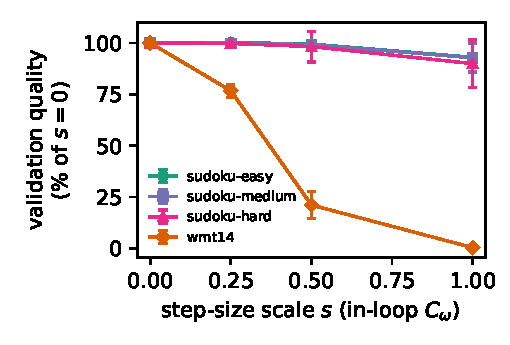
\includegraphics[width=\columnwidth]{figs/fig_dose.pdf}
\caption{Closed-loop validation quality of the in-loop corrector as a function of its step-size scale $s$ (relative to $s=0$, mean$\pm$std over five seeds; Sudoku: solve rate, WMT14: BLEU). Quality decreases monotonically with $s$; the effect is strongest for translation, where the generator is most sensitive to its input latent.}
\label{fig:dose}
\end{figure}

\subsection{Why in-loop correction fails: exposure to off-distribution inputs}
Figure~\ref{fig:dose} shows the closed-loop dose-response: validation quality decreases monotonically with the step-size scale. On WMT14 it drops to roughly three quarters of the baseline at $s=0.25$ and to almost zero at $s=1$. The open-loop objective~\eqref{eq:loss} rewards moving $\zh^{(k)}$ towards $\zh^{(k)}_{\mathrm{GT}}$ \emph{on average}, but the generator was trained only on inputs $u_{k+1}$ obtained from exact cumulative sums of codewords (clean or corrupted). A corrected latent is a continuous point that is closer in $\ell_2$ yet not of this form, and the generator's code predictions on such inputs are much worse. This is the exposure-bias mechanism~\citep{bengio2015scheduled,ross2011dagger}, and it is the failure mode anticipated in the caveat to Proposition~\ref{prop:contraction}: the bound holds at the error rate $\sigma_k$ of the \emph{corrected} process, which is far above that of NCM.

\textbf{On-manifold projection.} If exposure to non-lattice inputs is the cause, projecting the corrected latent back onto the lattice of codeword sums should remove most of the collapse. After applying $C_\omega$ at level $k$, we re-quantize the level-$k$ residual against $\mathcal{V}_k$, $\tilde r_k=\arg\min_v\|\mathrm{Down}_k(\zt^{(k)}-\zh^{(k-1)})-e_{k,v}\|_2$, and feed $\zh^{(k-1)}+\Phi_k(\Up_k(E_k(\tilde r_k)))$ to the generator, so every input is again a sum $\sum_{j\le k}\Phi_j\Up_jE_j(\cdot)$. On a 32-board Sudoku-hard check set (seed-42 correctors), projection raises the unselected in-loop corrector from \ProjNoSelOff\% to \ProjNoSelOn\% solved, against \ProjNCM\% for untouched NCM; for the validation-selected corrector it gives \ProjSelOn\% (\ProjSelOff\% without projection). This confirms the exposure-bias diagnosis. Projection still trails NCM because nearest-neighbor re-quantization of one level cannot recover the global constraint satisfaction that the generator's own codes encode.

\textbf{Closed-loop co-adaptation of the generator.} The remaining option is to adapt the generator to revised trajectories. Table~\ref{tab:dagger} fine-tunes the generator on the 400 training boards with teacher-forced reference states (control), with DAgger~\citep{ross2011dagger} on a 50/50 mix of reference and on-policy rollout states labelled by greedy residual quantization of $z-\text{state}$, and with DAgger plus a jointly trained in-loop $C_\omega$. No arm beats NCM. On Sudoku-hard the three arms reach \DgTfHard, \DgDagHard{} and \DgDagCHard\% (NCM \BaseHard\%; seed-mean $t$-test $p=\DgPTfHard$, $\DgPDagHard$, $\DgPDagCHard$), and on Sudoku-medium \DgTfMedium, \DgDagMedium{} and \DgDagCMedium\% (NCM 96.00\%). On Sudoku-easy all three arms are significantly \emph{worse} (\DgTfEasy, \DgDagEasy, \DgDagCEasy\% vs.\ 99.47\%, $p\le\DgPTfEasy$), because the 100-board validation set is saturated and cannot distinguish checkpoints. Validation accuracy decreases during fine-tuning on Sudoku-hard, and selection keeps the official model for one to three of five seeds on hard and medium. A few hundred boards cannot move the decision boundaries of a 25M-parameter generator that was fitted jointly with fixed codebooks during large-scale Stage-2 training; small-sample closed-loop adaptation overfits before it removes the shift.

\begin{table*}[t]
\centering
\caption{Closed-loop co-adaptation of the generator on Sudoku (1{,}500 held-out boards; 5 seeds). All arms fine-tune the 25.3M non-embedding generator parameters on the 400 training boards of $N_{\mathrm{tr}}$ for 3 rounds $\times$ 4 epochs (AdamW, lr $3{\times}10^{-5}$) and select the checkpoint by closed-loop solve rate on the 100 validation boards (the official model is a candidate). \emph{Control}: teacher-forced reference states. \emph{DAgger}: 50/50 reference and on-policy rollout states, labels given by greedy residual quantization of $z-\text{state}$. \emph{DAgger}+$C_\omega$: rollout states revised by a jointly trained in-loop corrector. Cells: solved \% mean$\pm$std (seed-mean $t$-test $p$ vs.\ NCM; number of seeds for which the official model was selected).}
\label{tab:dagger}
\setlength{\tabcolsep}{4pt}
\begin{tabular}{lcccc}
\toprule
 & NCM & Control (TF fine-tune) & DAgger & DAgger + $C_\omega$\\
\midrule
Sudoku-easy & 99.47 & 98.96$\pm$0.15 (0.002; 0/5) & 98.92$\pm$0.12 (5.1e-04; 0/5) & 99.04$\pm$0.14 (0.002; 0/5)\\
Sudoku-medium & 96.00 & 95.93$\pm$0.12 (0.266; 3/5) & 95.75$\pm$0.43 (0.261; 3/5) & 95.75$\pm$0.33 (0.162; 2/5)\\
Sudoku-hard & 86.67 & 85.87$\pm$1.10 (0.178; 3/5) & 86.27$\pm$0.58 (0.197; 2/5) & 86.27$\pm$0.96 (0.404; 1/5)\\
\bottomrule
\end{tabular}
\end{table*}


\begin{table*}[t]
\centering
\caption{Quality of the decoded intermediate latent $D_\psi(\zh^{(k)})$ (or $D_\psi(\zt^{(k)})$) at every level $k$, seed 42, test items. Fine-drop makes every level decodable, but quality rises steeply only over the last third of the hierarchy. WMT14 has 11 levels and XSum 9.}
\label{tab:levels}
\setlength{\tabcolsep}{2.6pt}
\begin{tabular}{llcccccccccccc}
\toprule
 & & \multicolumn{12}{c}{level $k$}\\
 & & 1 & 2 & 3 & 4 & 5 & 6 & 7 & 8 & 9 & 10 & 11 & 12\\
\midrule
Sudoku-hard cell acc. & NCM & 14.6 & 14.6 & 16.9 & 20.2 & 20.2 & 27.8 & 33.2 & 45.5 & 62.0 & 76.1 & 81.9 & 98.4\\
 & in-loop $C_\omega$ (no sel.) & 14.4 & 14.2 & 16.5 & 19.2 & 17.1 & 25.0 & 25.7 & 20.5 & 1.8 & 2.1 & 8.7 & 52.7\\
 & decode-path $C_\omega$ & 14.6 & 14.6 & 16.9 & 20.2 & 20.2 & 27.8 & 33.1 & 45.5 & 62.0 & 76.2 & 82.1 & 98.4\\
\midrule
Sudoku-hard solved & NCM & 0.0 & 0.0 & 0.0 & 0.0 & 0.0 & 0.0 & 0.0 & 0.0 & 0.0 & 0.0 & 0.0 & 86.7\\
 & in-loop $C_\omega$ (no sel.) & 0.0 & 0.0 & 0.0 & 0.0 & 0.0 & 0.0 & 0.0 & 0.0 & 0.0 & 0.0 & 0.0 & 17.9\\
 & decode-path $C_\omega$ & 0.0 & 0.0 & 0.0 & 0.0 & 0.0 & 0.0 & 0.0 & 0.0 & 0.0 & 0.0 & 0.0 & 86.7\\
\midrule
WMT14 BLEU & NCM & 0.4 & 0.9 & 1.6 & 2.9 & 5.0 & 7.6 & 12.3 & 15.4 & 17.7 & 19.2 & 22.3 & --\\
 & in-loop $C_\omega$ (no sel.) & 0.1 & 0.1 & 0.1 & 0.2 & 0.2 & 0.1 & 0.0 & 0.0 & 0.0 & 0.0 & 0.0 & --\\
 & decode-path $C_\omega$ & 0.4 & 0.9 & 1.5 & 2.8 & 5.0 & 7.6 & 12.3 & 15.4 & 17.7 & 19.2 & 22.3 & --\\
\midrule
XSum R-L & NCM & 19.2 & 21.7 & 23.0 & 23.6 & 24.5 & 25.4 & 26.1 & 26.4 & 27.6 & -- & -- & --\\
 & in-loop $C_\omega$ (no sel.) & 8.3 & 2.8 & 1.6 & 1.5 & 1.7 & 2.2 & 1.9 & 0.9 & 6.3 & -- & -- & --\\
 & decode-path $C_\omega$ & 19.2 & 21.7 & 23.0 & 23.6 & 24.5 & 25.4 & 26.1 & 26.4 & 27.6 & -- & -- & --\\
\bottomrule
\end{tabular}
\end{table*}


\subsection{Level-by-level decoding}
\label{sec:diag}
Table~\ref{tab:levels} and Figure~\ref{fig:levels} decode the latent after every level. Fine-drop training does make all levels decodable, but the information is concentrated in the last levels: on Sudoku-hard, cell accuracy is below 35\% up to level 7 (and no board is solved before the final level 12), and on WMT14 BLEU stays below 8 until level 6 and increases by more than 3 points at each of the last two levels. The decode-path corrector changes intermediate Sudoku cell accuracy by at most $0.57$ points (largest gains at levels 10--11 on Sudoku-easy and -medium, $\le0.22$ on Sudoku-hard) and lowers WMT14 BLEU by $0.10$--$0.13$ at levels 3--4, despite per-level scales selected on validation data. In-loop correction without selection lowers every level after the first few.

\begin{figure*}[t]
\centering
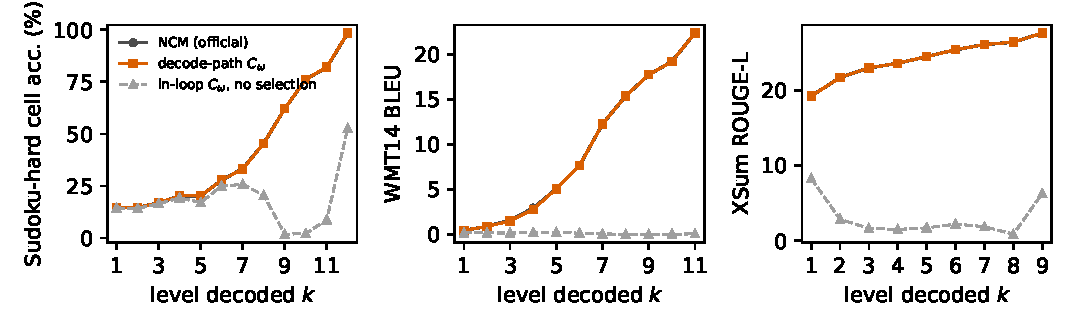
\includegraphics[width=\textwidth]{figs/fig_levels.pdf}
\caption{Quality of decoding at intermediate levels (seed 42, test items). Official NCM, decode-path corrector (overlapping NCM almost everywhere) and in-loop corrector without validation selection.}
\label{fig:levels}
\end{figure*}

\subsection{Halting trade-off}
\label{sec:halt}
Figure~\ref{fig:halt} and the top of Table~\ref{tab:sens} sweep $\tau$ on uncorrected latents. For small $\tau$ neither rule ever fires. When a rule does fire, it fires at an intermediate level whose decoding is poor: on all 2{,}000 Sudoku-hard boards the flux rule with $\tau=0.05$ stops after \ZsFluxFiveLevHard{} levels on average and solves \ZsFluxFiveHard\% (versus \ZsBaseHard\%), and the stability rule with $\tau=0.10$ stops after \ZsStabTenLevHard{} levels and solves \ZsStabTenHard\%. Figure~\ref{fig:flux} explains this behavior. The relative flux of the \emph{reference} latents is not monotone in $k$: on Sudoku-hard it drops to $0.045$ at level 5, where cell accuracy is only about 20\%, and rises again to above 0.4 at the fine levels. A threshold that lets the rule fire at all therefore fires at the coarse dip. On WMT14 the flux is never below 0.29. This is the empirical failure of Assumption~\ref{as:geo} quantified in Section~\ref{sec:theory}.

\begin{figure*}[t]
\centering
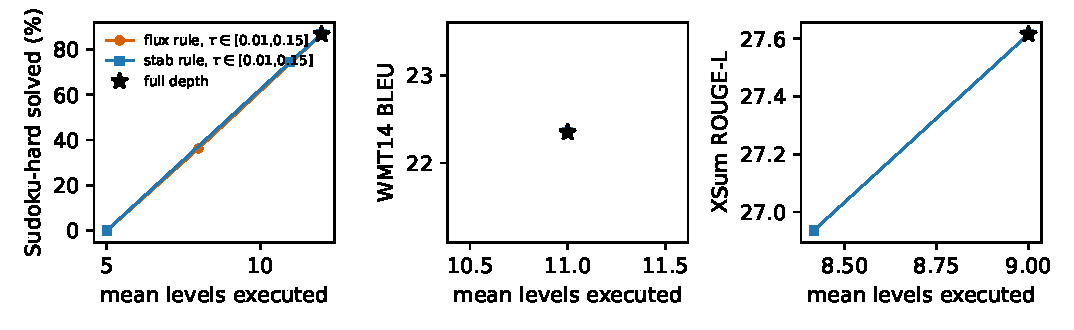
\includegraphics[width=\textwidth]{figs/fig_halt.pdf}
\caption{Quality versus mean executed levels for the flux and stability halting rules on uncorrected latents ($\tau\in\{0.01,\dots,0.15\}$, test items). Star: full depth. On WMT14 no setting halts; on XSum the stability rule at $\tau=0.15$ saves 0.6 levels on average at a cost of 0.7 ROUGE-L.}
\label{fig:halt}
\end{figure*}

\begin{figure}[t]
\centering
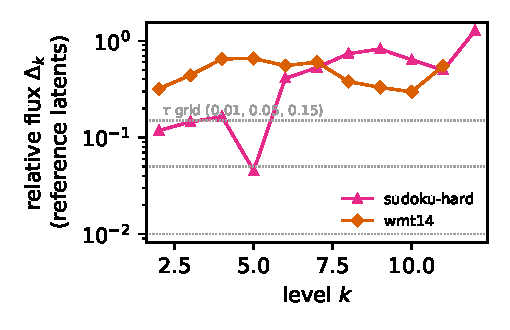
\includegraphics[width=\columnwidth]{figs/fig_flux.pdf}
\caption{Relative latent flux $\Delta_k$~\eqref{eq:flux} along reference trajectories of the released tokenizers (64 Sudoku-hard boards, 12 WMT14 sentences). Dotted lines mark the $\tau$ grid. The flux does not decay with $k$, which violates the premise of Proposition~\ref{prop:rd}.}
\label{fig:flux}
\end{figure}

\textbf{Token freezing.} At $\tau_{\mathrm{tok}}\le0.02$ fewer than 0.1\% of segments are ever frozen and outputs are unchanged. At $\tau_{\mathrm{tok}}=0.05$, 55\% of segments are frozen on Sudoku-hard and the solve rate drops from 86.7\% to 71.0\%; since freezing does not reduce FLOPs in the dense block-diagonal implementation, there is no setting with a favorable trade-off.

\begin{table}[t]
\centering
\caption{Sensitivity on Sudoku-hard (1{,}500 test boards; NCM: 86.7\% solved, 98.4\% cells). Top: halting threshold on uncorrected latents, cells give solved\,\% / $\bar k$ for the flux and stability rules. Middle and bottom: in-loop corrector with fixed $\eta_k$ (no step-size calibration) and different sizes (learned $\eta_k$, initialized at 0.5), seed 42, without and with validation checkpoint selection; columns give solved\,\%, cell\,\%, parameters, training time (s, 40 epochs on T4) and peak training memory (MB).}
\label{tab:sens}
\setlength{\tabcolsep}{2.4pt}
\begin{tabular}{lccccc}
\toprule
Setting & flux / solved & stab / cell & params & s & MB\\
\midrule
$\tau=0.01$ & 86.7 / 12.00 & 86.7 / 12.00 & -- & -- & --\\
$\tau=0.03$ & 86.7 / 12.00 & 86.7 / 12.00 & -- & -- & --\\
$\tau=0.05$ & 36.2 / 7.99 & 86.7 / 12.00 & -- & -- & --\\
$\tau=0.1$ & 0.0 / 5.00 & 74.4 / 10.97 & -- & -- & --\\
$\tau=0.15$ & 0.0 / 5.00 & 0.0 / 5.00 & -- & -- & --\\
\midrule
$\eta_k\equiv0.25$ (no sel.) & 17.4 & 52.5 & 1.23M & 127 & 3635\\
$\eta_k\equiv0.5$ (no sel.) & 10.5 & 41.7 & 1.23M & 127 & 3761\\
$\eta_k\equiv1.0$ (no sel.) & 44.3 & 73.8 & 1.23M & 127 & 2950\\
$\eta_k\equiv0.25$ (val.-sel.) & 86.4 & 98.3 & 1.23M & 122 & 1732\\
$\eta_k\equiv0.5$ (val.-sel.) & 86.5 & 98.4 & 1.23M & 122 & 1193\\
$\eta_k\equiv1.0$ (val.-sel.) & 86.4 & 98.4 & 1.23M & 122 & 820\\
\midrule
size 0.31M (no sel.) & 0.5 & 16.4 & 0.31M & 85 & 1560\\
size 1.23M (no sel.) & 17.9 & 52.7 & 1.23M & 127 & 3769\\
size 3.04M (no sel.) & 58.8 & 86.5 & 3.04M & 191 & 4360\\
size 0.31M (val.-sel.) & 62.5 & 89.3 & 0.31M & 82 & 813\\
size 1.23M (val.-sel.) & 86.5 & 98.4 & 1.23M & 122 & 812\\
size 3.04M (val.-sel.) & 86.9 & 98.4 & 3.04M & 181 & 834\\
\bottomrule
\end{tabular}
\end{table}


\textbf{Per-sequence margin halting with batch compaction.} Batch-lockstep halting forces the whole batch to wait for its hardest item, and raw flux has a coarse dip at level~5 (Fig.~\ref{fig:flux}). We therefore also implemented per-sequence halting with true batch compaction: each sequence halts individually for $k\ge8$ when its decoder top-1 margin $\mu_{i,k}=\min_t(p_{(1)}-p_{(2)})$ exceeds $\tau_{\mathrm{margin}}$ (Step~4 of Appendix~\ref{app:p2}) and its decoding is unchanged from level $k-1$, and halted sequences are removed from the active batch. The rule never fires for $\tau_{\mathrm{margin}}\in\{0.5,0.8,0.9,0.95\}$. Across 64 boards per difficulty, the share of boards whose level-$k$ decoding equals the final one is \MarginEqMax\% for every $k\le11$, between \FlipsMin{} and \FlipsMax{} cells still change at the last level, and the median margin at level~11 is at most \MarginMedMax. Task resolution is concentrated in the final level, so no lossless early exit exists for these checkpoints at any granularity.

\subsection{Sensitivity}
Table~\ref{tab:sens} varies the step size and the corrector size for the in-loop corrector on Sudoku-hard. Without validation selection, all configurations are far below NCM, and larger correctors are less harmful (0.31M: 0.5\%, 3.04M: 58.8\% solved). We attribute this to the zero-initialized output projection: a larger model fits the identity on rollout trajectories more closely. With validation checkpoint selection, the 1.23M and 3.04M correctors reach 86.4--86.9\% solved, within 0.2 points of NCM, while the 0.31M corrector reaches only 62.5\%. Training a 1.2M-parameter corrector for 40 epochs on 500 boards takes about two minutes on the T4 with at most 4.4\,GB peak memory (all sizes), and building the training trajectories takes 16\,s.

\begin{figure*}[t]\centering\scriptsize\setlength{\tabcolsep}{4pt}
\begin{tabular}{lcccc}
\toprule & level 3 & level 6 & level 9 & level 12\\\midrule
NCM & \texttt{\begin{tabular}{@{}c@{}}5 2 6 4 7 4 7 3 6\\3 7 1 3 7 1 2 9 6\\8 7 1 2 7 8 2 9 6\\2 3 7 8 2 6 1 7 6\\6 5 7 5 8 7 1 2 4\\2 4 7 9 2 6 8 6 4\\7 1 3 7 1 4 2 8 8\\7 8 3 7 3 4 6 7 9\\7 6 2 7 8 4 4 4 9\end{tabular}} & \texttt{\begin{tabular}{@{}c@{}}5 2 2 4 7 8 7 9 9\\9 9 9 4 3 3 2 3 2\\3 7 6 4 7 1 7 5 5\\5 5 5 5 8 7 8 7 4\\8 8 3 5 6 7 1 4 4\\4 4 4 9 2 6 3 3 3\\5 4 5 7 6 4 6 6 8\\6 6 6 7 8 5 4 5 5\\5 6 5 5 3 7 4 4 7\end{tabular}} & \texttt{\begin{tabular}{@{}c@{}}5 6 5 4 4 2 2 9 1\\1 7 9 8 6 5 5 2 2\\2 2 4 9 1 1 6 8 8\\7 5 6 9 1 4 3 3 2\\8 3 3 9 2 6 1 1 4\\4 1 1 1 3 7 9 5 5\\7 4 3 1 5 5 2 2 8\\9 1 1 6 8 3 5 4 4\\6 8 5 4 4 7 3 1 1\end{tabular}} & \texttt{\begin{tabular}{@{}c@{}}5 6 8 4 3 2 7 9 1\\9 7 1 8 6 5 4 2 3\\2 3 4 7 9 1 6 8 5\\7 5 6 9 1 4 8 3 2\\8 9 3 5 2 6 1 7 4\\4 1 2 3 7 8 9 5 6\\3 4 7 1 5 9 2 6 8\\1 2 9 6 8 3 5 4 7\\6 8 5 2 4 7 3 1 9\end{tabular}}\\\midrule
in-loop $C_\omega$ (no sel.) & \texttt{\begin{tabular}{@{}c@{}}5 2 2 4 4 4 4 8 8\\8 4 1 3 3 8 5 5 6\\8 7 6 2 7 8 2 4 6\\8 8 8 8 2 6 8 8 6\\5 5 7 5 8 7 4 2 4\\2 4 7 8 4 6 5 5 4\\7 4 5 4 8 4 2 4 2\\4 8 4 7 6 8 5 5 5\\8 8 2 8 8 4 4 4 9\end{tabular}} & \texttt{\begin{tabular}{@{}c@{}}5 2 2 3 3 . 9 9 9\\9 9 9 1 3 3 2 2 2\\3 3 6 1 6 5 4 5 5\\5 . 5 . 5 . 8 8 .\\8 8 6 . 6 1 . 4 4\\. 4 4 2 3 3 3 3 3\\5 3 . 3 6 . 1 6 6\\6 6 6 6 8 . 4 5 5\\5 6 5 5 3 2 4 4 6\end{tabular}} & \texttt{\begin{tabular}{@{}c@{}}. . . 4 . . . . .\\. . . . . . . 4 .\\2 . . . . . . . .\\. 5 . . 1 . . . .\\. 5 . . . . . . 4\\. . . . . . . . .\\. . . . . . . . 8\\. . . . . . . . .\\. . . 4 . . . . .\end{tabular}} & \texttt{\begin{tabular}{@{}c@{}}5 6 8 4 3 2 7 9 1\\9 7 1 8 6 5 4 2 3\\2 3 4 7 9 1 6 8 5\\7 5 6 9 1 4 8 3 2\\8 3 5 2 6 1 7 4 4\\1 2 3 7 8 9 5 6 3\\4 7 1 5 9 2 6 8 1\\2 9 6 8 3 5 4 7 6\\8 5 2 4 7 3 1 9 .\end{tabular}}\\
\bottomrule\end{tabular}
\caption{Intermediate decodings of Sudoku-hard test board 500 (seed 42). Both samplers produce near-identical coarse boards; the in-loop corrector perturbs the generator input from level 6 on and the final board is wrong, while NCM solves it. A dot marks a position whose decoded token is not a digit.}
\label{fig:qual}\end{figure*}

\subsection{Qualitative case study and failure modes}
Figure~\ref{fig:qual} shows the intermediate boards of a Sudoku-hard puzzle that NCM solves and the unselected in-loop corrector does not. At level 3 the two samplers agree; after the correction perturbs the generator input at the middle levels, the later codes diverge and the final board contains errors. We observed three failure modes in total. (i) \emph{Closed-loop distribution shift}: in-loop correction moves latents towards the reference in $\ell_2$ but off the set of codeword sums the generator was trained on (Figure~\ref{fig:dose}). (ii) \emph{Premature halting at a coarse flux dip}: on Sudoku-hard the reference flux at level 5 is lower than at any fine level (Figure~\ref{fig:flux}), so any $\tau$ large enough to stop early stops at a level whose decoding solves almost no board; on Sudoku-medium the flux rule with $\tau=0.15$ stops after \ZsFluxFifteenLevMedium{} levels and solves \ZsFluxFifteenMedium\% of boards. (iii) \emph{No margin for a decode-path corrector}: because the final-level decoding is already the decoder's training input, the best decode-path correction at level $K$ is the identity.

\subsection{Limitations}
Our study has several limitations. Unconditional generation (TinyStories, LM1B, OWT) is outside the reference-based scope of this study, the validation-selected in-loop corrector was not run on XSum, and generator co-adaptation was run on Sudoku only. The splits are drawn from the official test files because no released validation inputs exist, which reduces test-set size. Only greedy decoding was studied; stochastic decoding might leave more room for correction. The corrector was trained on a few hundred to a thousand items; a larger training set, or co-training the generator on corrected latents (a DAgger-style scheme~\citep{ross2011dagger}), might remove the distribution shift but would require training the generator, which is outside the frozen-checkpoint protocol of this paper. Finally, the halting rules use simple norm and stability statistics; a learned halting head trained on the level-wise decoding quality could exploit information the flux does not capture.

\section{Conclusion and Pre-Training Prescriptions}
We asked whether predictor-corrector latent revision and adaptive early halting can improve frozen coarse-to-fine next-concept models without retraining them. Propositions~\ref{prop:contraction} and~\ref{prop:rd} give the conditions: closed-loop contraction of the corrector on the generator's support, and geometric decay of latent increments with terminal margin. Bit-exact experiments on five official checkpoints show that standard MS-RVQ pre-training violates all three requirements. The generator is brittle off the lattice of codeword sums. Fine-drop makes intermediate latents decodable but does not make increments contract. Task resolution is concentrated in the final level. Every variant we tried, including in-loop, decode-path and projected correction, batch and per-sequence halting, token freezing and DAgger co-adaptation of the generator, fails to improve on NCM under held-out selection.

The propositions also indicate what pre-training would have to change. (i) \emph{Residual-decay regularization in Stage~1}: penalizing $\max\big(0,\|\Delta\zh^{(k)}_{\mathrm{GT}}\|_F-\rho\|\Delta\zh^{(k-1)}_{\mathrm{GT}}\|_F\big)$ for a target $\rho<1$ during MS-RVQ training would make Assumption~\ref{as:geo} hold by construction and give halting a non-vacuous budget, at a possible cost in final reconstruction. (ii) \emph{Continuous latent perturbation in Stage~2}: adding Gaussian perturbations of the cumulative latent to the input of every level during generator pre-training, in addition to discrete code corruption, would make the generator locally Lipschitz off the codeword lattice, which is the property a closed-loop contractive corrector needs. Both changes require retraining the released models and are left to future work; the released harness allows them to be tested under the same protocol.



\section*{Broader Impact Statement}
This work studies inference-time modifications of publicly released text-generation models on puzzle solving, translation and summarization benchmarks. It does not introduce new models, data or capabilities, and its main finding is that the studied modifications do not improve the released models. We do not foresee direct negative societal consequences beyond those of the underlying generators.

\section*{Reproducibility Statement}
All experiments use the unmodified official code, checkpoints and datasets of the evaluated models and run on a single 16\,GB GPU. The harness, Kaggle job scripts, per-run result files, per-item predictions and the scripts that generate every table and figure from these files are available at \url{https://github.com/TashfikS/ncm-posthoc-revision-halting}; implementation and protocol details are given in Appendix~\ref{app:repro}.

\bibliography{refs}
\bibliographystyle{tmlr}

\appendix
\section{Proof of Proposition~\ref{prop:contraction}}
\label{app:p1}
\textit{Step 1 (drift recursion).} By~\eqref{eq:cum} and~\eqref{eq:pred}, $\zh^{(k)}-\zh^{(k)}_{\mathrm{GT}}=\zh^{(k-1)}-\zh^{(k-1)}_{\mathrm{GT}}+A_k\big(E_k(\hat r_k)-E_k(r_k^\ast)\big)$, i.e., $e^{(k)}=e^{(k-1)}+\epsilon_k$ with $e^{(0)}=0$.

\textit{Step 2 (one-step lower bound).} Let $a=\|e^{(k-1)}\|$ and $b=\|\epsilon_k\|$. By Assumption~\ref{as:coh},
\begin{equation}
\|e^{(k)}\|^2=a^2+2\langle e^{(k-1)},\epsilon_k\rangle+b^2\ge a^2+2c_0ab+b^2.
\end{equation}
Since $c_0\le1$, $a^2+2c_0ab+b^2\ge a^2+2c_0ab+c_0^2b^2=(a+c_0b)^2$, so $\|e^{(k)}\|\ge\|e^{(k-1)}\|+c_0\|\epsilon_k\|$.

\textit{Step 3 (telescoping).} Summing Step 2 over $k=1,\dots,K$ yields $\|e^{(K)}\|\ge c_0\sum_{k=1}^K\|\epsilon_k\|$. Taking expectations and using $\sigma_k=\mathbb{E}\|\epsilon_k\|$ gives~\eqref{eq:lower}.

\textit{Step 4 (size of $\sigma_k$).} $E_k(\hat r_k)-E_k(r_k^\ast)$ has at most $m_k$ non-zero rows, each of norm at most $\mathrm{diam}(\mathcal{V}_k)=\max_{v,v'}\|e_{k,v}-e_{k,v'}\|$; hence its Frobenius norm is at most $\sqrt{m_k}\,\mathrm{diam}(\mathcal{V}_k)\le m_k\,\mathrm{diam}(\mathcal{V}_k)$, and Assumption~\ref{as:lip} gives $\|\epsilon_k\|\le L_p m_k\mathrm{diam}(\mathcal{V}_k)$. Note that $\Up_k$ replicates each coarse row over about $L/\ell_k$ fine rows; for linear interpolation $\|\Up_k\|_{\mathrm{op}}\le\sqrt{\lceil L/\ell_k\rceil}$, so $L_p$ is largest at coarse levels, which is the broadcast effect described in Section~IV-A.

\textit{Step 5 (corrected recursion).} With the in-loop corrector, $\zt^{(k)}=\mathcal{C}_k\big(\zt^{(k-1)}+A_kE_k(\hat r_k)\big)$, where $\hat r_k$ are the codes produced by the generator when it is conditioned on $\zt^{(k-1)}$, and $\epsilon_k=A_k(E_k(\hat r_k)-E_k(r^\ast_k))$ with $\sigma_k=\mathbb{E}\|\epsilon_k\|$ for this process. Using $\zh^{(k)}_{\mathrm{GT}}=\zh^{(k-1)}_{\mathrm{GT}}+A_kE_k(r^\ast_k)$ from~\eqref{eq:cum},
\begin{align}
&\zt^{(k-1)}+A_kE_k(\hat r_k)-\zh^{(k)}_{\mathrm{GT}}\nonumber\\
&\quad=\big(\zt^{(k-1)}-\zh^{(k-1)}_{\mathrm{GT}}\big)+A_k\big(E_k(\hat r_k)-E_k(r^\ast_k)\big)\nonumber\\
&\quad=\tilde e^{(k-1)}+\epsilon_k.
\end{align}
Assumption~\ref{as:corr} (valid because the iterate stays in the radius-$R$ ball) then gives
\begin{align}
V_k&\le(1-\gamma_k)\|\tilde e^{(k-1)}+\epsilon_k\|+\epsilon_{\mathrm{corr}}\nonumber\\
&\le(1-\gamma_k)(V_{k-1}+\|\epsilon_k\|)+\epsilon_{\mathrm{corr}}.
\end{align}

\textit{Step 6 (unrolling).} We claim $V_k\le\sum_{i=1}^{k}\big(\prod_{j=i}^{k}(1-\gamma_j)\big)\|\epsilon_i\|+\epsilon_{\mathrm{corr}}\sum_{i=1}^{k}\prod_{j=i+1}^{k}(1-\gamma_j)$, with the empty product equal to 1. For $k=1$, $V_0=0$ gives $V_1\le(1-\gamma_1)\|\epsilon_1\|+\epsilon_{\mathrm{corr}}$. If the claim holds for $k-1$, inserting it into Step 5 and multiplying out by $(1-\gamma_k)$ gives the claim for $k$. Taking expectations at $k=K$ yields~\eqref{eq:upper}.

\textit{Step 7 (uniform bound).} If $\gamma_j\ge\gamma$ and $\sigma_k\le\bar\sigma$, then $\prod_{j=i}^{K}(1-\gamma_j)\le(1-\gamma)^{K-i+1}$ and $\sum_{i=1}^{K}(1-\gamma)^{K-i+1}\le(1-\gamma)/\gamma$, $\sum_{i=1}^{K}(1-\gamma)^{K-i}\le1/\gamma$. Hence $\mathbb{E}V_K\le\bar\sigma(1-\gamma)/\gamma+\epsilon_{\mathrm{corr}}/\gamma$. \hfill$\blacksquare$

\textit{Caveat.} Step 5 conditions on the generator's errors \emph{after} correction. If the corrector moves $\zt^{(k-1)}$ off the generator's training distribution, $\sigma_k$ in~\eqref{eq:upper} can be much larger than in the uncorrected process; the bound does not compare the two processes at equal $\sigma_k$. This is the mechanism behind the closed-loop failure in Section~\ref{sec:results}.

\section{Proof of Proposition~\ref{prop:rd}}
\label{app:p2}
\textit{Step 1 (Cauchy tail).} By the triangle inequality, $\|\zt^{(K)}-\zt^{(k^\ast)}\|=\|\sum_{j=k^\ast+1}^{K}\Delta\zt^{(j)}\|\le\sum_{j=k^\ast+1}^{K}\|\Delta\zt^{(j)}\|$. Assumption~\ref{as:geo} gives $\|\Delta\zt^{(k^\ast+m)}\|\le\rho^m\|\Delta\zt^{(k^\ast)}\|\le\rho^m\tau$, so the sum is at most $\tau\sum_{m\ge1}\rho^m=\rho\tau/(1-\rho)\le\tau/(1-\rho)$.

\textit{Step 2 (KL between softmaxes).} Let $\Lambda(a)=\log\sum_v e^{a_v}$ and $p_a=\nabla\Lambda(a)=\mathrm{softmax}(a)$. Direct computation gives $\KL(p_a\|p_b)=\Lambda(b)-\Lambda(a)-\langle p_a,b-a\rangle$, the Bregman divergence of $\Lambda$. By Taylor's theorem with integral remainder, $\KL(p_a\|p_b)=\int_0^1(1-s)\,h^\top\nabla^2\Lambda(a+sh)\,h\,ds$ with $h=b-a$. Since $\nabla^2\Lambda(c)=\mathrm{diag}(p_c)-p_cp_c^\top$, $h^\top\nabla^2\Lambda(c)h=\mathrm{Var}_{v\sim p_c}(h_v)\le\mathbb{E}_{p_c}h_v^2\le\|h\|_\infty^2\le\|h\|_2^2$. Therefore $\KL(p_a\|p_b)\le\frac12\|a-b\|_2^2$.

\textit{Step 3 (sum over positions).} Applying Step 2 to every position $t$ with $a_t=f(\zt^{(K)})_t$ and $b_t=f(\zt^{(k^\ast)})_t$ and summing, $\sum_t\KL\le\frac12\|f(\zt^{(K)})-f(\zt^{(k^\ast)})\|_F^2\le\frac{L_D^2}{2}\|\zt^{(K)}-\zt^{(k^\ast)}\|^2$ by Assumption~\ref{as:dec}. Inserting Step 1 gives $\sum_t\KL\le L_D^2\tau^2/(2(1-\rho)^2)$. \hfill$\blacksquare$

\textit{Step 4 (argmax preservation).} By Pinsker's inequality, $\mathrm{TV}_t\le\sqrt{\KL^{(t)}/2}\le L_D\tau/(2(1-\rho))$ at every position, where $\KL^{(t)}$ is the KL divergence at position $t$. If the full-depth distribution has top-1 margin $\mu_t=p_{(1)}-p_{(2)}>2\,\mathrm{TV}_t$, the top-1 token cannot change, so the halted output equals the full-depth output at position $t$.

\section{Reproducibility details}
\label{app:repro}
\textit{Harness.} The official \texttt{generate()} is executed unmodified. We wrap \texttt{MultiscaleResidualVectorQuantizer.}\allowbreak\texttt{get\_next\_autoregressive\_input}, which \texttt{generate()} calls once per level, to (i) record $\zh^{(k)}$, (ii) apply $C_\omega$, (iii) apply token freezing, and (iv) raise an exception that unwinds the official loop when the halting test fires. Without a corrector, halting or freezing, the wrapped sampler reproduces the official \texttt{eval\_shard.py} latent exactly (maximum absolute difference $0.0$ and identical code indices on Sudoku-hard). The output of the final level is formed as in \texttt{idx\_to\_zhats}. Decoded token ids are converted to strings with the official \texttt{dec()} and, for XSum, the official frequency-penalized \texttt{pick\_tokens()}.

\textit{Metrics.} Sudoku exact match and cell accuracy reproduce \texttt{eval\_merge.exact}; BLEU~\citep{papineni2002bleu} is \texttt{sacrebleu.corpus\_bleu}~\citep{post2018sacrebleu} on detokenized strings; ROUGE uses \texttt{rouge\_score} with stemming~\citep{lin2004rouge}. Paired tests use per-item cell accuracy (Sudoku), sentence BLEU (WMT14) or ROUGE-L (XSum) for the Wilcoxon signed-rank test~\citep{wilcoxon1945}, the exact McNemar test~\citep{mcnemar1947} on per-board solved indicators, and a one-sample $t$-test of the five seed means against the deterministic baseline.

\textit{FLOPs.} FLOPs per sequence are measured with \texttt{torch.utils.flop\_counter.FlopCounterMode} on one batch of the evaluation set for every possible number of executed levels, including the corrector, the decoder and, for halting, the criterion evaluation; the per-configuration value is read at the mean number of executed levels.

\section{Architecture overview}
\label{app:arch}
Figure~\ref{fig:arch} contrasts baseline NCM and APC-NCM.

\begin{figure*}[t]
\centering
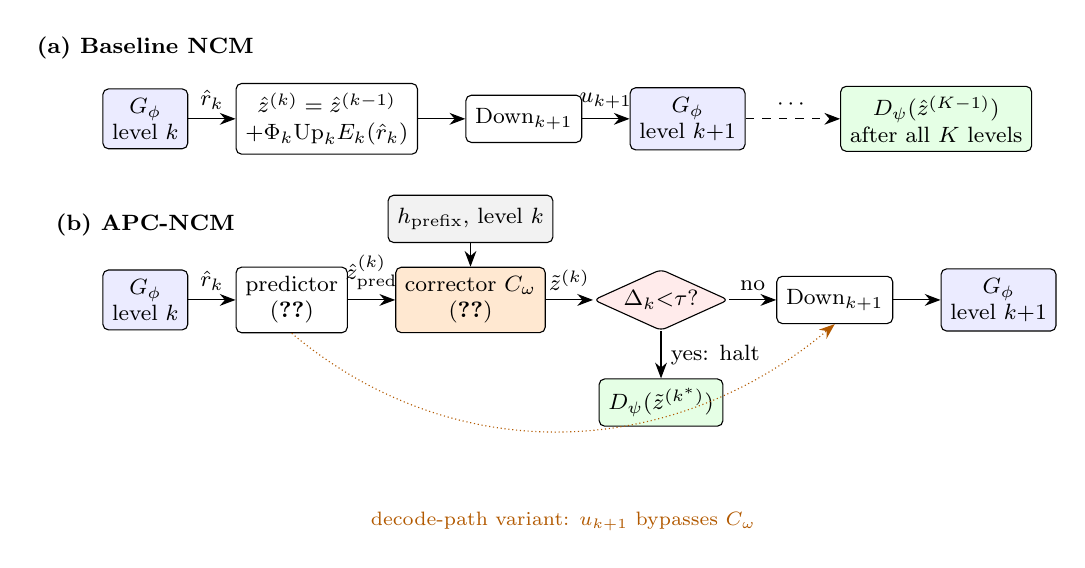
\begin{tikzpicture}[font=\footnotesize, node distance=4mm and 6mm,
 box/.style={draw, rounded corners=2pt, minimum height=6mm, align=center, fill=white},
 gen/.style={box, fill=blue!8}, cor/.style={box, fill=orange!18}, dec/.style={box, fill=green!10}, hal/.style={box, fill=red!8, diamond, aspect=2.2, inner sep=1pt},
 >={Stealth[length=2mm]}]
\node[font=\bfseries\footnotesize] (tA) at (0,0.9) {(a) Baseline NCM};
\node[gen] (g0) at (0,0) {$G_\phi$\\level $k$};
\node[box, right=of g0] (p0) {$\zh^{(k)}=\zh^{(k-1)}$\\$+\Phi_k\Up_k E_k(\hat r_k)$};
\node[box, right=of p0] (d0) {$\mathrm{Down}_{k+1}$};
\node[gen, right=of d0] (g1) {$G_\phi$\\level $k{+}1$};
\node[dec, right=12mm of g1] (o0) {$D_\psi(\zh^{(K-1)})$\\after all $K$ levels};
\draw[->] (g0) -- node[above]{$\hat r_k$} (p0); \draw[->] (p0) -- (d0); \draw[->] (d0) -- node[above]{$u_{k+1}$} (g1); \draw[->, dashed] (g1) -- node[above]{$\cdots$} (o0);
\node[font=\bfseries\footnotesize] (tB) at (0,-1.35) {(b) APC-NCM};
\node[gen] (G0) at (0,-2.3) {$G_\phi$\\level $k$};
\node[box, right=of G0] (P0) {predictor\\ \eqref{eq:pred}};
\node[cor, right=of P0] (C0) {corrector $C_\omega$\\ \eqref{eq:corr}};
\node[hal, right=of C0] (H0) {$\Delta_k{<}\tau$?};
\node[box, right=of H0] (D0) {$\mathrm{Down}_{k+1}$};
\node[gen, right=of D0] (G1) {$G_\phi$\\level $k{+}1$};
\node[dec, below=6mm of H0] (O0) {$D_\psi(\zt^{(k^\ast)})$};
\node[box, above=3mm of C0, fill=gray!10] (pf) {$h_{\mathrm{prefix}}$, level $k$};
\draw[->] (G0) -- node[above]{$\hat r_k$} (P0); \draw[->] (P0) -- node[above]{$\zh^{(k)}_{\mathrm{pred}}$} (C0); \draw[->] (C0) -- node[above]{$\zt^{(k)}$} (H0);
\draw[->] (H0) -- node[above]{no} (D0); \draw[->] (D0) -- (G1); \draw[->] (H0) -- node[right]{yes: halt} (O0); \draw[->] (pf) -- (C0);
\draw[->, densely dotted, orange!70!black] (P0.south) to[out=-40,in=-140] node[below=9mm, pos=0.5, font=\scriptsize, text=orange!70!black]{decode-path variant: $u_{k+1}$ bypasses $C_\omega$} (D0.south);
\end{tikzpicture}
\caption{Baseline NCM (a) adds one quantized residual per level and always runs all $K$ levels. APC-NCM (b) revises the cumulative latent with a learned corrector and may halt once the latent flux (or decoder instability) falls below $\tau$. In the in-loop variant the corrected latent feeds the next generator level; in the decode-path variant (dotted) the generator continues from the uncorrected latent and $C_\omega$ acts only on decoded latents.}
\label{fig:arch}
\end{figure*}

\section{Algorithm}
\label{app:alg}
Algorithm~\ref{alg:apc} summarizes training and inference.

\begin{algorithm}[t]
\caption{APC-NCM training and inference}
\label{alg:apc}
\begin{algorithmic}[1]
\Require frozen $E_\theta,D_\psi,\{\mathcal{V}_k,\Phi_k\}$, $G_\phi$; training inputs/references $\{(c_i,y_i)\}_{i\le N_{\mathrm{tr}}}$
\State \textbf{Training}
\For{$i=1,\dots,N_{\mathrm{tr}}$}
  \State $(\zh^{(k)}_{\mathrm{GT}})_k\gets$ \texttt{z\_to\_idx}$(E_\theta(y_i))$;\quad $(\zh^{(k)}_{\mathrm{roll}})_k\gets$ greedy rollout of $G_\phi$ on $c_i$
  \State $(\zh^{(k)}_{\mathrm{cor}})_k\gets$ cumulative latents of codes corrupted at rate $u\sim\mathcal{U}(0,1)$, level 0 kept
\EndFor
\State minimize~\eqref{eq:loss} with AdamW, one-cycle LR; keep best validation epoch (identity included)
\State choose $s$ (or $s_k$) by closed-loop validation quality; choose rule and $\tau$ on $\{c_i\}$
\State \textbf{Inference} on a batch of prefixes $c$
\State $\zh^{(-1)}\gets 0$; sample $\hat r_0$ with $G_\phi$
\For{$k=0,\dots,K-2$}
  \State $\zh^{(k)}\gets\zh^{(k-1)}+\Phi_k\Up_kE_k(\hat r_k)$ \Comment{predictor}
  \State $\zt^{(k)}\gets\zh^{(k)}-\eta_kC_\omega(\zh^{(k)},h_{\mathrm{prefix}},k)$ \Comment{corrector}
  \If{freezing} copy rows of $\zh^{(k-1)}$ into frozen segments \EndIf
  \If{$k\ge k_{\min}$ \textbf{and} halting criterion holds for all sequences} \Return $D_\psi(\zt^{(k)})$ \EndIf
  \State $u_{k+1}\gets\mathrm{Down}_{k+1}(\zt^{(k)})$ (in-loop) or $\mathrm{Down}_{k+1}(\zh^{(k)})$ (decode-path)
  \State $\hat r_{k+1}\gets\argmax G_\phi(u_{k+1},c)$
\EndFor
\State \Return $D_\psi\big(\zh^{(K-2)}{+}\Phi_{K-1}E_{K-1}(\hat r_{K-1})\big)$, corrected at level $K{-}1$ in the decode-path variant
\end{algorithmic}
\end{algorithm}

\section{Hardware, profiling and hyper-parameters}
\label{app:hw}
\textbf{Hardware and profiling.} Every number comes from Kaggle Tesla T4 (16\,GB, 14.6\,GB usable) sessions with Python 3.13 and the preinstalled PyTorch~\citep{paszke2019pytorch} CUDA build. Wall-clock latency is the mean over evaluation batches after one untimed warm-up batch, synchronized with \texttt{torch.cuda.synchronize}; peak memory is \texttt{torch.cuda.max\_memory\_allocated}. Variants of the same task were timed in the same session. Hyper-parameters are listed in Table~\ref{tab:hp}.

\begin{table}[t]
\centering
\caption{Hyper-parameters. Generator and tokenizer settings are those of the official evaluation configs.}
\label{tab:hp}
\footnotesize\setlength{\tabcolsep}{2.5pt}
\begin{tabular}{lccc}
\toprule
 & Sudoku & WMT14 & XSum\\
\midrule
levels $K$ & 12 & 11 & 9\\
$L$, $d$ & 89, 256 & 64, 768 & 48, 768\\
generator params & 25.5M & 120.0M & 88.0M\\
$C_\omega$ params (width) & 1.23M & 1.20M & 1.20M\\
train / test items & 500 / 1500 & 1000 / 2003 & 500 / 1000\\
epochs & 40 & 20 & 30\\
batch (train / eval) & 32 / 128 & 32 / 64 & 32 / 32\\
optimizer & \multicolumn{3}{c}{AdamW~\citep{loshchilov2019adamw}, lr $3{\times}10^{-4}$, wd 0.01, one-cycle, clip 1.0}\\
$\alpha$ (KL weight) & \multicolumn{3}{c}{0.1}\\
$\eta_k$ init / scale grid & \multicolumn{3}{c}{$\sigma(\beta_k)=0.5$ / $s\in\{0,0.25,0.5,1\}$}\\
rollout / corruption mix & \multicolumn{3}{c}{0.75 / 0.25 (2 corrupted copies, $u\sim\mathcal{U}(0,1)$)}\\
$\tau$ grid, $k_{\min}$ & \multicolumn{3}{c}{\{0.01,0.03,0.05,0.10,0.15\}, 2}\\
$\tau_{\mathrm{tok}}$ grid & \multicolumn{3}{c}{\{0.005,0.01,0.02,0.05\}}\\
selection tolerance & \multicolumn{3}{c}{0.5 points of full-depth quality}\\
seeds & \multicolumn{3}{c}{42, 0, 1, 2, 3}\\
\bottomrule
\end{tabular}
\end{table}


\section{Small-sample generator co-adaptation}
\label{app:dag_small}
\textbf{Closed-loop co-adaptation of the generator.} The remaining option is to adapt the generator to revised trajectories. Table~\ref{tab:dagger} fine-tunes the generator on the 400 training boards with teacher-forced reference states (control), with DAgger~\citep{ross2011dagger} on a 50/50 mix of reference and on-policy rollout states labelled by greedy residual quantization of $z-\text{state}$, and with DAgger plus a jointly trained in-loop $C_\omega$. No arm beats NCM. On Sudoku-hard the three arms reach \DgTfHard, \DgDagHard{} and \DgDagCHard\% (NCM \BaseHard\%; seed-mean $t$-test $p=\DgPTfHard$, $\DgPDagHard$, $\DgPDagCHard$), and on Sudoku-medium \DgTfMedium, \DgDagMedium{} and \DgDagCMedium\% (NCM 96.00\%). On Sudoku-easy all three arms are significantly \emph{worse} (\DgTfEasy, \DgDagEasy, \DgDagCEasy\% vs.\ 99.47\%, $p\le\DgPTfEasy$), because the 100-board validation set is saturated and cannot distinguish checkpoints. Validation accuracy decreases during fine-tuning on Sudoku-hard, and selection keeps the official model for one to three of five seeds on hard and medium. A few hundred boards cannot move the decision boundaries of a 25M-parameter generator that was fitted jointly with fixed codebooks during large-scale Stage-2 training; small-sample closed-loop adaptation overfits before it removes the shift. With 30$\times$ more training boards (Section~\ref{sec:scaled}, Table~\ref{tab:dagaug}) the loss on easy disappears, but there is still no significant gain.

\begin{table*}[t]
\centering
\caption{Closed-loop co-adaptation of the generator on Sudoku (1{,}500 held-out boards; 5 seeds). All arms fine-tune the 25.3M non-embedding generator parameters on the 400 training boards of $N_{\mathrm{tr}}$ for 3 rounds $\times$ 4 epochs (AdamW, lr $3{\times}10^{-5}$) and select the checkpoint by closed-loop solve rate on the 100 validation boards (the official model is a candidate). \emph{Control}: teacher-forced reference states. \emph{DAgger}: 50/50 reference and on-policy rollout states, labels given by greedy residual quantization of $z-\text{state}$. \emph{DAgger}+$C_\omega$: rollout states revised by a jointly trained in-loop corrector. Cells: solved \% mean$\pm$std (seed-mean $t$-test $p$ vs.\ NCM; number of seeds for which the official model was selected).}
\label{tab:dagger}
\setlength{\tabcolsep}{4pt}
\begin{tabular}{lcccc}
\toprule
 & NCM & Control (TF fine-tune) & DAgger & DAgger + $C_\omega$\\
\midrule
Sudoku-easy & 99.47 & 98.96$\pm$0.15 (0.002; 0/5) & 98.92$\pm$0.12 (5.1e-04; 0/5) & 99.04$\pm$0.14 (0.002; 0/5)\\
Sudoku-medium & 96.00 & 95.93$\pm$0.12 (0.266; 3/5) & 95.75$\pm$0.43 (0.261; 3/5) & 95.75$\pm$0.33 (0.162; 2/5)\\
Sudoku-hard & 86.67 & 85.87$\pm$1.10 (0.178; 3/5) & 86.27$\pm$0.58 (0.197; 2/5) & 86.27$\pm$0.96 (0.404; 1/5)\\
\bottomrule
\end{tabular}
\end{table*}


\section{Level-by-level decoding table}
\label{app:levels}
\begin{table*}[t]
\centering
\caption{Quality of the decoded intermediate latent $D_\psi(\zh^{(k)})$ (or $D_\psi(\zt^{(k)})$) at every level $k$, seed 42, test items. Fine-drop makes every level decodable, but quality rises steeply only over the last third of the hierarchy. WMT14 has 11 levels and XSum 9.}
\label{tab:levels}
\setlength{\tabcolsep}{2.6pt}
\begin{tabular}{llcccccccccccc}
\toprule
 & & \multicolumn{12}{c}{level $k$}\\
 & & 1 & 2 & 3 & 4 & 5 & 6 & 7 & 8 & 9 & 10 & 11 & 12\\
\midrule
Sudoku-hard cell acc. & NCM & 14.6 & 14.6 & 16.9 & 20.2 & 20.2 & 27.8 & 33.2 & 45.5 & 62.0 & 76.1 & 81.9 & 98.4\\
 & in-loop $C_\omega$ (no sel.) & 14.4 & 14.2 & 16.5 & 19.2 & 17.1 & 25.0 & 25.7 & 20.5 & 1.8 & 2.1 & 8.7 & 52.7\\
 & decode-path $C_\omega$ & 14.6 & 14.6 & 16.9 & 20.2 & 20.2 & 27.8 & 33.1 & 45.5 & 62.0 & 76.2 & 82.1 & 98.4\\
\midrule
Sudoku-hard solved & NCM & 0.0 & 0.0 & 0.0 & 0.0 & 0.0 & 0.0 & 0.0 & 0.0 & 0.0 & 0.0 & 0.0 & 86.7\\
 & in-loop $C_\omega$ (no sel.) & 0.0 & 0.0 & 0.0 & 0.0 & 0.0 & 0.0 & 0.0 & 0.0 & 0.0 & 0.0 & 0.0 & 17.9\\
 & decode-path $C_\omega$ & 0.0 & 0.0 & 0.0 & 0.0 & 0.0 & 0.0 & 0.0 & 0.0 & 0.0 & 0.0 & 0.0 & 86.7\\
\midrule
WMT14 BLEU & NCM & 0.4 & 0.9 & 1.6 & 2.9 & 5.0 & 7.6 & 12.3 & 15.4 & 17.7 & 19.2 & 22.3 & --\\
 & in-loop $C_\omega$ (no sel.) & 0.1 & 0.1 & 0.1 & 0.2 & 0.2 & 0.1 & 0.0 & 0.0 & 0.0 & 0.0 & 0.0 & --\\
 & decode-path $C_\omega$ & 0.4 & 0.9 & 1.5 & 2.8 & 5.0 & 7.6 & 12.3 & 15.4 & 17.7 & 19.2 & 22.3 & --\\
\midrule
XSum R-L & NCM & 19.2 & 21.7 & 23.0 & 23.6 & 24.5 & 25.4 & 26.1 & 26.4 & 27.6 & -- & -- & --\\
 & in-loop $C_\omega$ (no sel.) & 8.3 & 2.8 & 1.6 & 1.5 & 1.7 & 2.2 & 1.9 & 0.9 & 6.3 & -- & -- & --\\
 & decode-path $C_\omega$ & 19.2 & 21.7 & 23.0 & 23.6 & 24.5 & 25.4 & 26.1 & 26.4 & 27.6 & -- & -- & --\\
\bottomrule
\end{tabular}
\end{table*}


\section{Further halting variants}
\label{app:halt_extra}
\textbf{Token freezing.} At $\tau_{\mathrm{tok}}\le0.02$ fewer than 0.1\% of segments are ever frozen and outputs are unchanged. At $\tau_{\mathrm{tok}}=0.05$, 55\% of segments are frozen on Sudoku-hard and the solve rate drops from 86.7\% to 71.0\%; since freezing does not reduce FLOPs in the dense block-diagonal implementation, there is no setting with a favorable trade-off.

\textbf{Per-sequence margin halting with batch compaction.} Batch-lockstep halting forces the whole batch to wait for its hardest item, and raw flux has a coarse dip at level~5 (Fig.~\ref{fig:flux}). We therefore also implemented per-sequence halting with true batch compaction: each sequence halts individually for $k\ge8$ when its decoder top-1 margin $\mu_{i,k}=\min_t(p_{(1)}-p_{(2)})$ exceeds $\tau_{\mathrm{margin}}$ (Step~4 of Appendix~\ref{app:p2}) and its decoding is unchanged from level $k-1$, and halted sequences are removed from the active batch. The rule never fires for $\tau_{\mathrm{margin}}\in\{0.5,0.8,0.9,0.95\}$. Across 64 boards per difficulty, the share of boards whose level-$k$ decoding equals the final one is \MarginEqMax\% for every $k\le11$, between \FlipsMin{} and \FlipsMax{} cells still change at the last level, and the median margin at level~11 is at most \MarginMedMax. Task resolution is concentrated in the final level, so no lossless early exit exists for these checkpoints at any granularity.

\section{Sensitivity and qualitative analysis}
\label{app:sens}
\begin{table}[t]
\centering
\caption{Sensitivity on Sudoku-hard (1{,}500 test boards; NCM: 86.7\% solved, 98.4\% cells). Top: halting threshold on uncorrected latents, cells give solved\,\% / $\bar k$ for the flux and stability rules. Middle and bottom: in-loop corrector with fixed $\eta_k$ (no step-size calibration) and different sizes (learned $\eta_k$, initialized at 0.5), seed 42, without and with validation checkpoint selection; columns give solved\,\%, cell\,\%, parameters, training time (s, 40 epochs on T4) and peak training memory (MB).}
\label{tab:sens}
\setlength{\tabcolsep}{2.4pt}
\begin{tabular}{lccccc}
\toprule
Setting & flux / solved & stab / cell & params & s & MB\\
\midrule
$\tau=0.01$ & 86.7 / 12.00 & 86.7 / 12.00 & -- & -- & --\\
$\tau=0.03$ & 86.7 / 12.00 & 86.7 / 12.00 & -- & -- & --\\
$\tau=0.05$ & 36.2 / 7.99 & 86.7 / 12.00 & -- & -- & --\\
$\tau=0.1$ & 0.0 / 5.00 & 74.4 / 10.97 & -- & -- & --\\
$\tau=0.15$ & 0.0 / 5.00 & 0.0 / 5.00 & -- & -- & --\\
\midrule
$\eta_k\equiv0.25$ (no sel.) & 17.4 & 52.5 & 1.23M & 127 & 3635\\
$\eta_k\equiv0.5$ (no sel.) & 10.5 & 41.7 & 1.23M & 127 & 3761\\
$\eta_k\equiv1.0$ (no sel.) & 44.3 & 73.8 & 1.23M & 127 & 2950\\
$\eta_k\equiv0.25$ (val.-sel.) & 86.4 & 98.3 & 1.23M & 122 & 1732\\
$\eta_k\equiv0.5$ (val.-sel.) & 86.5 & 98.4 & 1.23M & 122 & 1193\\
$\eta_k\equiv1.0$ (val.-sel.) & 86.4 & 98.4 & 1.23M & 122 & 820\\
\midrule
size 0.31M (no sel.) & 0.5 & 16.4 & 0.31M & 85 & 1560\\
size 1.23M (no sel.) & 17.9 & 52.7 & 1.23M & 127 & 3769\\
size 3.04M (no sel.) & 58.8 & 86.5 & 3.04M & 191 & 4360\\
size 0.31M (val.-sel.) & 62.5 & 89.3 & 0.31M & 82 & 813\\
size 1.23M (val.-sel.) & 86.5 & 98.4 & 1.23M & 122 & 812\\
size 3.04M (val.-sel.) & 86.9 & 98.4 & 3.04M & 181 & 834\\
\bottomrule
\end{tabular}
\end{table}



Table~\ref{tab:sens} varies the step size and the corrector size for the in-loop corrector on Sudoku-hard. Without validation selection, all configurations are far below NCM, and larger correctors are less harmful (0.31M: 0.5\%, 3.04M: 58.8\% solved). We attribute this to the zero-initialized output projection: a larger model fits the identity on rollout trajectories more closely. With validation checkpoint selection, the 1.23M and 3.04M correctors reach 86.4--86.9\% solved, within 0.2 points of NCM, while the 0.31M corrector reaches only 62.5\%. Training a 1.2M-parameter corrector for 40 epochs on 500 boards takes about two minutes on the T4 with at most 4.4\,GB peak memory (all sizes), and building the training trajectories takes 16\,s.

\begin{figure*}[t]\centering\scriptsize\setlength{\tabcolsep}{4pt}
\begin{tabular}{lcccc}
\toprule & level 3 & level 6 & level 9 & level 12\\\midrule
NCM & \texttt{\begin{tabular}{@{}c@{}}5 2 6 4 7 4 7 3 6\\3 7 1 3 7 1 2 9 6\\8 7 1 2 7 8 2 9 6\\2 3 7 8 2 6 1 7 6\\6 5 7 5 8 7 1 2 4\\2 4 7 9 2 6 8 6 4\\7 1 3 7 1 4 2 8 8\\7 8 3 7 3 4 6 7 9\\7 6 2 7 8 4 4 4 9\end{tabular}} & \texttt{\begin{tabular}{@{}c@{}}5 2 2 4 7 8 7 9 9\\9 9 9 4 3 3 2 3 2\\3 7 6 4 7 1 7 5 5\\5 5 5 5 8 7 8 7 4\\8 8 3 5 6 7 1 4 4\\4 4 4 9 2 6 3 3 3\\5 4 5 7 6 4 6 6 8\\6 6 6 7 8 5 4 5 5\\5 6 5 5 3 7 4 4 7\end{tabular}} & \texttt{\begin{tabular}{@{}c@{}}5 6 5 4 4 2 2 9 1\\1 7 9 8 6 5 5 2 2\\2 2 4 9 1 1 6 8 8\\7 5 6 9 1 4 3 3 2\\8 3 3 9 2 6 1 1 4\\4 1 1 1 3 7 9 5 5\\7 4 3 1 5 5 2 2 8\\9 1 1 6 8 3 5 4 4\\6 8 5 4 4 7 3 1 1\end{tabular}} & \texttt{\begin{tabular}{@{}c@{}}5 6 8 4 3 2 7 9 1\\9 7 1 8 6 5 4 2 3\\2 3 4 7 9 1 6 8 5\\7 5 6 9 1 4 8 3 2\\8 9 3 5 2 6 1 7 4\\4 1 2 3 7 8 9 5 6\\3 4 7 1 5 9 2 6 8\\1 2 9 6 8 3 5 4 7\\6 8 5 2 4 7 3 1 9\end{tabular}}\\\midrule
in-loop $C_\omega$ (no sel.) & \texttt{\begin{tabular}{@{}c@{}}5 2 2 4 4 4 4 8 8\\8 4 1 3 3 8 5 5 6\\8 7 6 2 7 8 2 4 6\\8 8 8 8 2 6 8 8 6\\5 5 7 5 8 7 4 2 4\\2 4 7 8 4 6 5 5 4\\7 4 5 4 8 4 2 4 2\\4 8 4 7 6 8 5 5 5\\8 8 2 8 8 4 4 4 9\end{tabular}} & \texttt{\begin{tabular}{@{}c@{}}5 2 2 3 3 . 9 9 9\\9 9 9 1 3 3 2 2 2\\3 3 6 1 6 5 4 5 5\\5 . 5 . 5 . 8 8 .\\8 8 6 . 6 1 . 4 4\\. 4 4 2 3 3 3 3 3\\5 3 . 3 6 . 1 6 6\\6 6 6 6 8 . 4 5 5\\5 6 5 5 3 2 4 4 6\end{tabular}} & \texttt{\begin{tabular}{@{}c@{}}. . . 4 . . . . .\\. . . . . . . 4 .\\2 . . . . . . . .\\. 5 . . 1 . . . .\\. 5 . . . . . . 4\\. . . . . . . . .\\. . . . . . . . 8\\. . . . . . . . .\\. . . 4 . . . . .\end{tabular}} & \texttt{\begin{tabular}{@{}c@{}}5 6 8 4 3 2 7 9 1\\9 7 1 8 6 5 4 2 3\\2 3 4 7 9 1 6 8 5\\7 5 6 9 1 4 8 3 2\\8 3 5 2 6 1 7 4 4\\1 2 3 7 8 9 5 6 3\\4 7 1 5 9 2 6 8 1\\2 9 6 8 3 5 4 7 6\\8 5 2 4 7 3 1 9 .\end{tabular}}\\
\bottomrule\end{tabular}
\caption{Intermediate decodings of Sudoku-hard test board 500 (seed 42). Both samplers produce near-identical coarse boards; the in-loop corrector perturbs the generator input from level 6 on and the final board is wrong, while NCM solves it. A dot marks a position whose decoded token is not a digit.}
\label{fig:qual}\end{figure*}

\paragraph{Qualitative case study and failure modes.}
Figure~\ref{fig:qual} shows the intermediate boards of a Sudoku-hard puzzle that NCM solves and the unselected in-loop corrector does not. At level 3 the two samplers agree; after the correction perturbs the generator input at the middle levels, the later codes diverge and the final board contains errors. We observed three failure modes in total. (i) \emph{Closed-loop distribution shift}: in-loop correction moves latents towards the reference in $\ell_2$ but off the set of codeword sums the generator was trained on (Figure~\ref{fig:dose}). (ii) \emph{Premature halting at a coarse flux dip}: on Sudoku-hard the reference flux at level 5 is lower than at any fine level (Figure~\ref{fig:flux}), so any $\tau$ large enough to stop early stops at a level whose decoding solves almost no board; on Sudoku-medium the flux rule with $\tau=0.15$ stops after \ZsFluxFifteenLevMedium{} levels and solves \ZsFluxFifteenMedium\% of boards. (iii) \emph{No margin for a decode-path corrector}: because the final-level decoding is already the decoder's training input, the best decode-path correction at level $K$ is the identity.

\section{On-manifold projection (small-sample runs)}
\label{app:proj}
\textbf{On-manifold projection.} If exposure to non-lattice inputs is the cause, projecting the corrected latent back onto the lattice of codeword sums should remove most of the collapse. After applying $C_\omega$ at level $k$, we re-quantize the level-$k$ residual against $\mathcal{V}_k$, $\tilde r_k=\arg\min_v\|\mathrm{Down}_k(\zt^{(k)}-\zh^{(k-1)})-e_{k,v}\|_2$, and feed $\zh^{(k-1)}+\Phi_k(\Up_k(E_k(\tilde r_k)))$ to the generator, so every input is again a sum $\sum_{j\le k}\Phi_j\Up_jE_j(\cdot)$. On a 32-board Sudoku-hard check set (seed-42 correctors), projection raises the unselected in-loop corrector from \ProjNoSelOff\% to \ProjNoSelOn\% solved, against \ProjNCM\% for untouched NCM; for the validation-selected corrector it gives \ProjSelOn\% (\ProjSelOff\% without projection). This confirms the exposure-bias diagnosis. Projection still trails NCM because nearest-neighbor re-quantization of one level cannot recover the global constraint satisfaction that the generator's own codes encode.

\section{Halting sweep}
\label{app:haltfig}
\begin{figure*}[t]
\centering
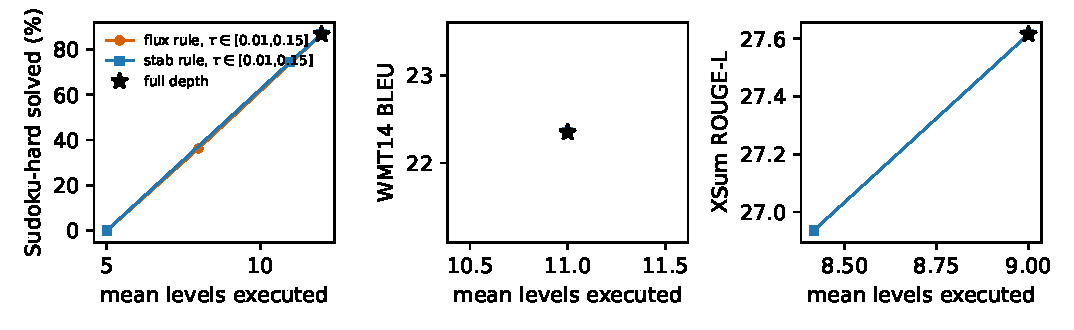
\includegraphics[width=\textwidth]{figs/fig_halt.pdf}
\caption{Quality versus mean executed levels for the flux and stability halting rules on uncorrected latents ($\tau\in\{0.01,\dots,0.15\}$, test items). Star: full depth. On WMT14 no setting halts; on XSum the stability rule at $\tau=0.15$ saves 0.6 levels on average at a cost of 0.7 ROUGE-L.}
\label{fig:halt}
\end{figure*}

\section{Additional figures and tables}
\label{app:extra_figs}
\begin{figure}[t]
\centering
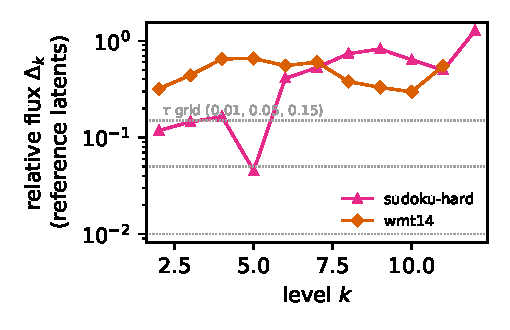
\includegraphics[width=\columnwidth]{figs/fig_flux.pdf}
\caption{Relative latent flux $\Delta_k$~\eqref{eq:flux} along reference trajectories of the released tokenizers (64 Sudoku-hard boards, 12 WMT14 sentences). Dotted lines mark the $\tau$ grid. The flux does not decay with $k$, which violates the premise of Proposition~\ref{prop:rd}.}
\label{fig:flux}
\end{figure}

\begin{figure}[t]\centering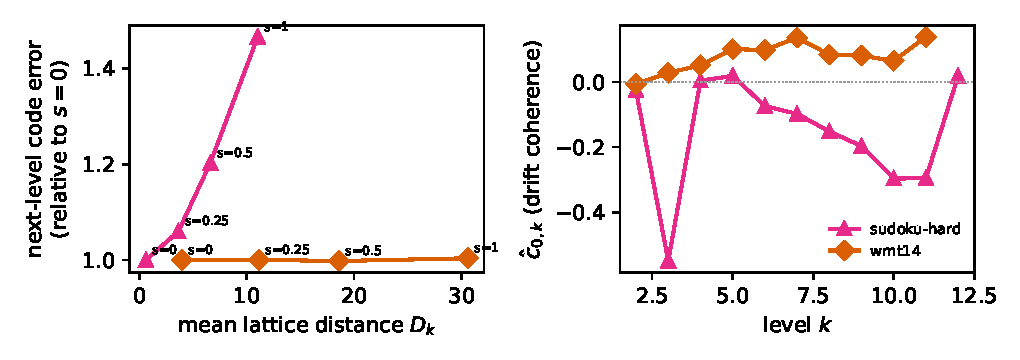
\includegraphics[width=0.85\linewidth]{figs/fig_offmanifold.pdf}
\caption{Measured constants of the revised Proposition~\ref{prop:contraction}. Left: next-level code error versus mean lattice distance when rollout states are revised by the in-loop corrector at step-size scale $s$ (seed-42 corrector). Right: per-level drift coherence $\hat c_{0,k}$ on greedy rollouts; negative values mean finer levels partially cancel accumulated drift.}\label{fig:offm}\end{figure}

\begin{figure}[t]
\centering
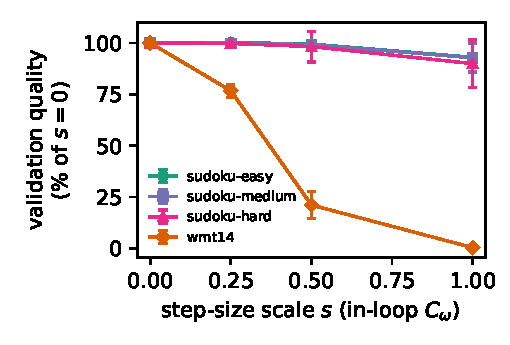
\includegraphics[width=\columnwidth]{figs/fig_dose.pdf}
\caption{Closed-loop validation quality of the in-loop corrector as a function of its step-size scale $s$ (relative to $s=0$, mean$\pm$std over five seeds; Sudoku: solve rate, WMT14: BLEU). Quality decreases monotonically with $s$; the effect is strongest for translation, where the generator is most sensitive to its input latent.}
\label{fig:dose}
\end{figure}

\begin{table*}[t]
\centering
\caption{Generator co-adaptation with 12{,}000 symmetry-augmented training boards (4 DAgger rounds of 1{,}000 fresh boards; checkpoint and corrector selected on 1{,}200 augmented validation boards; 1{,}500 held-out test boards; five seeds). Columns per arm: mean$\pm$std solve rate, one-sample $t$-test of seed means against NCM, smallest per-seed McNemar $p$, and the number of seeds for which validation selection kept the official generator.}
\label{tab:dagaug}
\small
\resizebox{\textwidth}{!}{\begin{tabular}{lc cccc cccc}
\toprule
& & \multicolumn{4}{c}{DAgger} & \multicolumn{4}{c}{DAgger + $C_\omega$}\\
\cmidrule(lr){3-6}\cmidrule(lr){7-10}
Task & NCM & solved & $t$-test $p$ & min.\ McN.\ $p$ & kept & solved & $t$-test $p$ & min.\ McN.\ $p$ & kept\\
\midrule
Sudoku-hard & 86.67 & 87.16$\pm$0.53 & 0.11 & 0.02 & 0/5 & 87.13$\pm$0.53 & 0.12 & 0.07 & 0/5 \\
Sudoku-medium & 96.00 & 95.71$\pm$0.27 & 0.07 & 0.29 & 2/5 & 95.92$\pm$0.17 & 0.36 & 0.59 & 1/5 \\
\bottomrule
\end{tabular}}
\end{table*}




\end{document}
